

\chapter{Additional discussions}
\label{c:misc}
\section{Quantum information approaches}
\label{s:QuanInfo}
\index{Quantum information}
Quantum information science has undergone enormous developments in the last 30 years. I do not treat this wide and fascinating field here, but shall only discuss briefly some relations with the question of formalism. Indeed information theory leads to new ways to consider and use  quantum theory. This renewal is sometimes considered as a real change of paradigm.

The interest in the relations between Information Theory and Quantum Physics started really in the 70's from several questions and results:
\begin{itemize}
  \item The relations and conflicts between General Relativity and Quantum Physics: the theoretical discovery of the Bekenstein-Hawking quantum entropy for black holes, the black hole evaporation (information) paradox, the more general Unruh effect and quantum  thermodynamical aspects of gravity and of events horizons (with many recent developments in quantum gravity and string theories, such as ``Holographic gravity'', ``Entropic Gravity'', etc.).
  \item The general ongoing discussions on the various interpretations of the quantum formalism, the meaning of quantum measurement processes, and whether a quantum state represent the ``reality'', or some ``element of reality'' on a quantum system, or simply the observer's information on the quantum system.
  \item Of course the theoretical and experimental developments of quantum computing. See for instance \cite{Nielsen:2010fk}. It started from the realization that quantum entanglement and quantum correlations can be used as a resource for performing calculations and the transmission of information in a more efficient way than when using classical correlations with classical channels.
   \item This led for instance to the famous ``It from Bit'' idea (or aphorism) of J. A. Wheeler (see e.g. in \cite{Zurek:1990fk})
and others (see for instance the book by Deutsch \cite{Deutsch:1997fk}, or talks by Fuchs \cite{Fuchs-2001,Fuchs-2002}). Roughly speaking this amounts to reverse the famous statement of Laudauer ``Information is Physics'' into ``Physics is Information'', and to state that Information is the good starting point to understand the nature of the physical world and of the physical laws. 
\end{itemize}

This point of view has been developed and advocated by several authors in the area of quantum gravity and quantum cosmology. 
Here I shall just mention some old or recent attempts to use this point of view to discuss the formalism of ``standard'' quantum physics, not taking into account the issues of quantum gravity.

In the quantum information inspired approaches a basic concept is that of %``quantum channel'', or 
``device'', or ``operation'', which represents the most general manipulation on a quantum system. In a very oversimplified presentation\footnote{slightly more general than in some presentations}, such a device  is a ``black box'' with both a quantum input system A and  quantum output system B, and with a set $I$ of classical settings $i\in I$ and a set $O$ of classical responses $o\in O$. 
\index{Quantum device}
%
%The input and the output may be in different ``states'' (quantum). 
%The state for the output $B$ depends on the classical response  $o\in O$. 
The input and output systems $A$ and $B$ may be different, and may be multipartite systems, e.g. may consist in collections of independent subsystems $A=\mathop\cup\limits_\alpha A_\alpha$, $B=\mathop\cup\limits_\alpha B_\beta$.

This general concept of device encompass the standard concepts of \emph{state} and of \emph{effect}.
\index{State (preparation)}\index{Effect}
A \emph{state} corresponds to the preparation of a quantum system $S$ in a definite state; there is no input $A=\emptyset$, the setting $i$ specify the state, there is no response, and  $B=S$ is the system.
An \emph{effect}, corresponds to a destructive measurement on a quantum system $S$;  the input $A=S$ is the system, there are no output $B=\emptyset$, no settings $i$, and the response set $O$ is the set of possible output measurements $o$.
This concept of device contains also the general concept of a \emph{quantum channel};  then $A=B$, there are no settings or responses.
%Finally to any thus constructed 
\begin{figure}[h]
\begin{center}
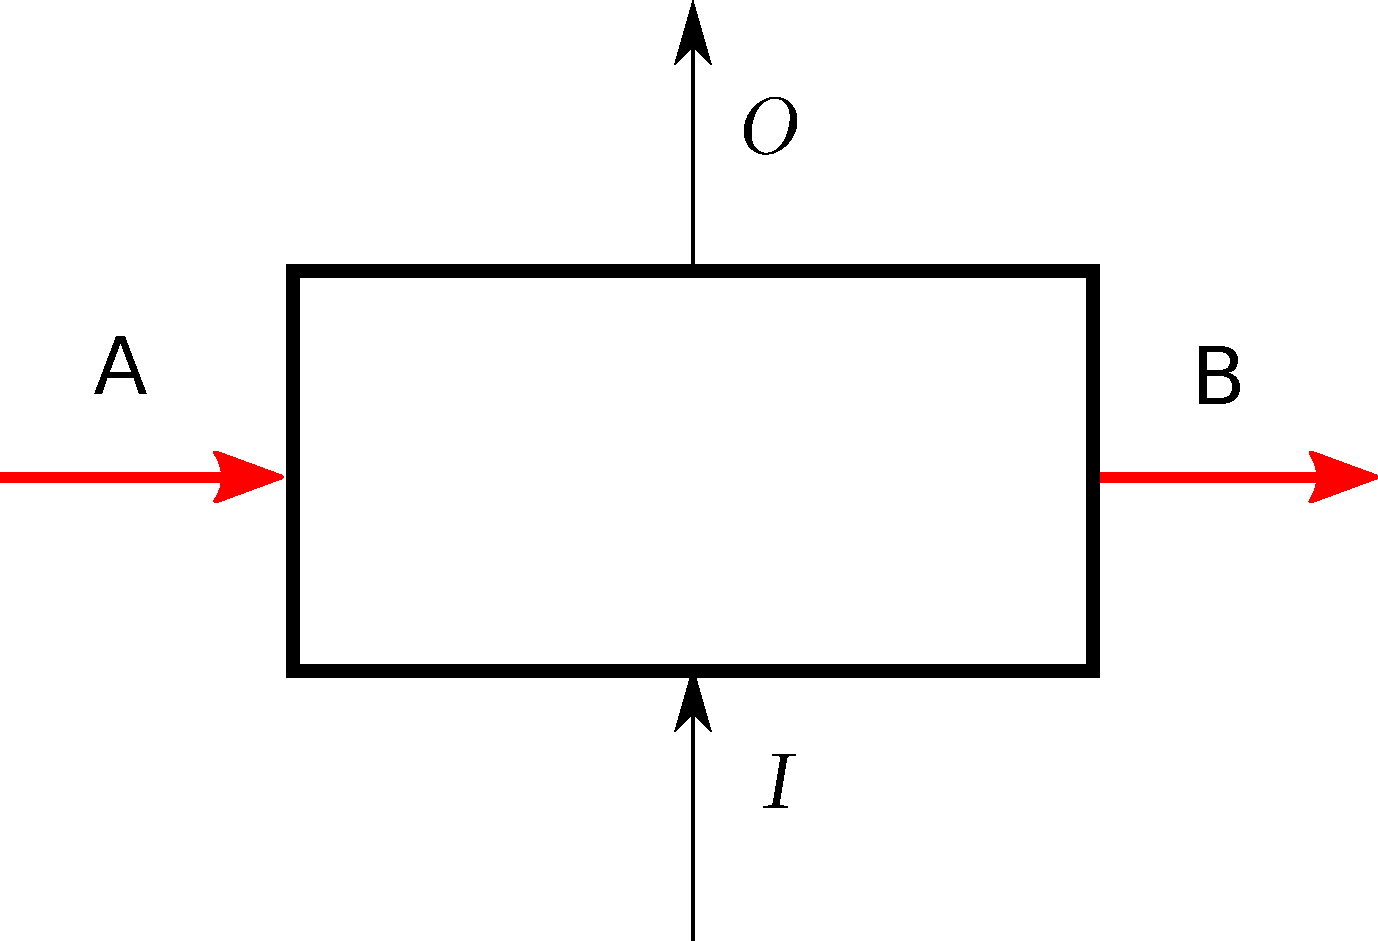
\includegraphics[width=2in]{quantum-test.pdf}
\qquad
\raisebox{-.9ex}{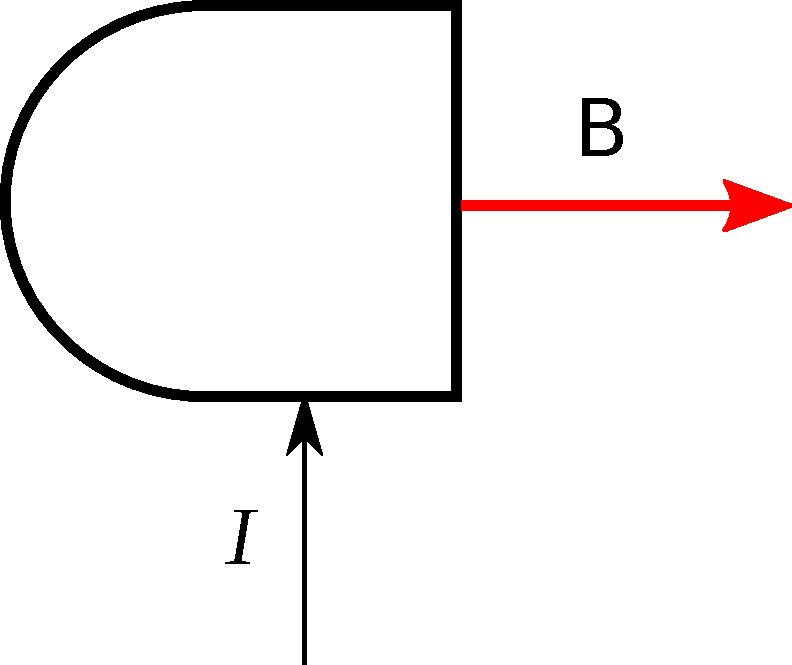
\includegraphics[width=1.2in]{quantum-state.pdf}}
\qquad
\raisebox{4.ex}{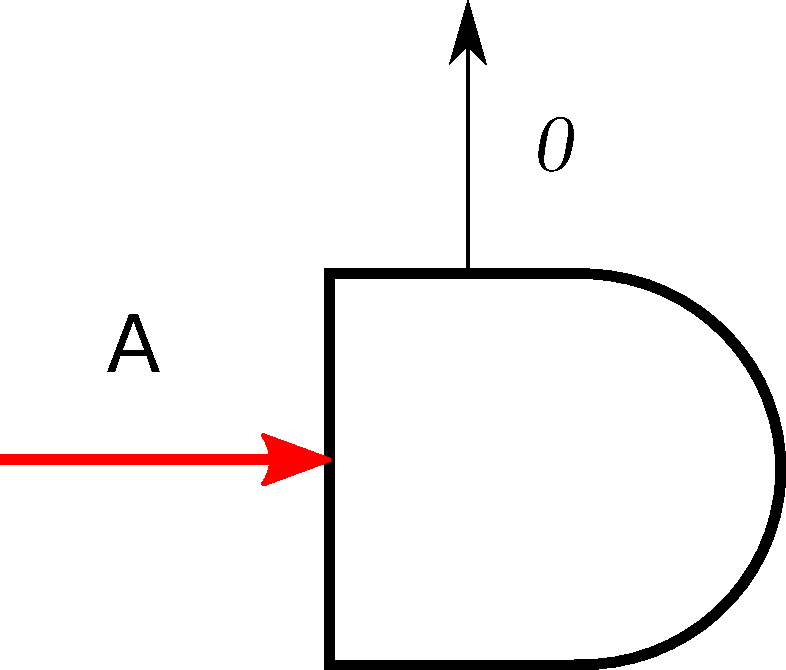
\includegraphics[width=1.2in]{quantum-effect.pdf}}
\caption{A general device, a state and an effect }
\label{fdevice}
\end{center}
\end{figure}
\index{Probabilities}
Probabilities $p(i | o)$  are associated to the combination of a state and an effect, this correspond to the standard concept of probability of observing some outcome $o$ when making a measurement on a quantum state (labeled by $i$).
\begin{figure}[h]
\begin{center}
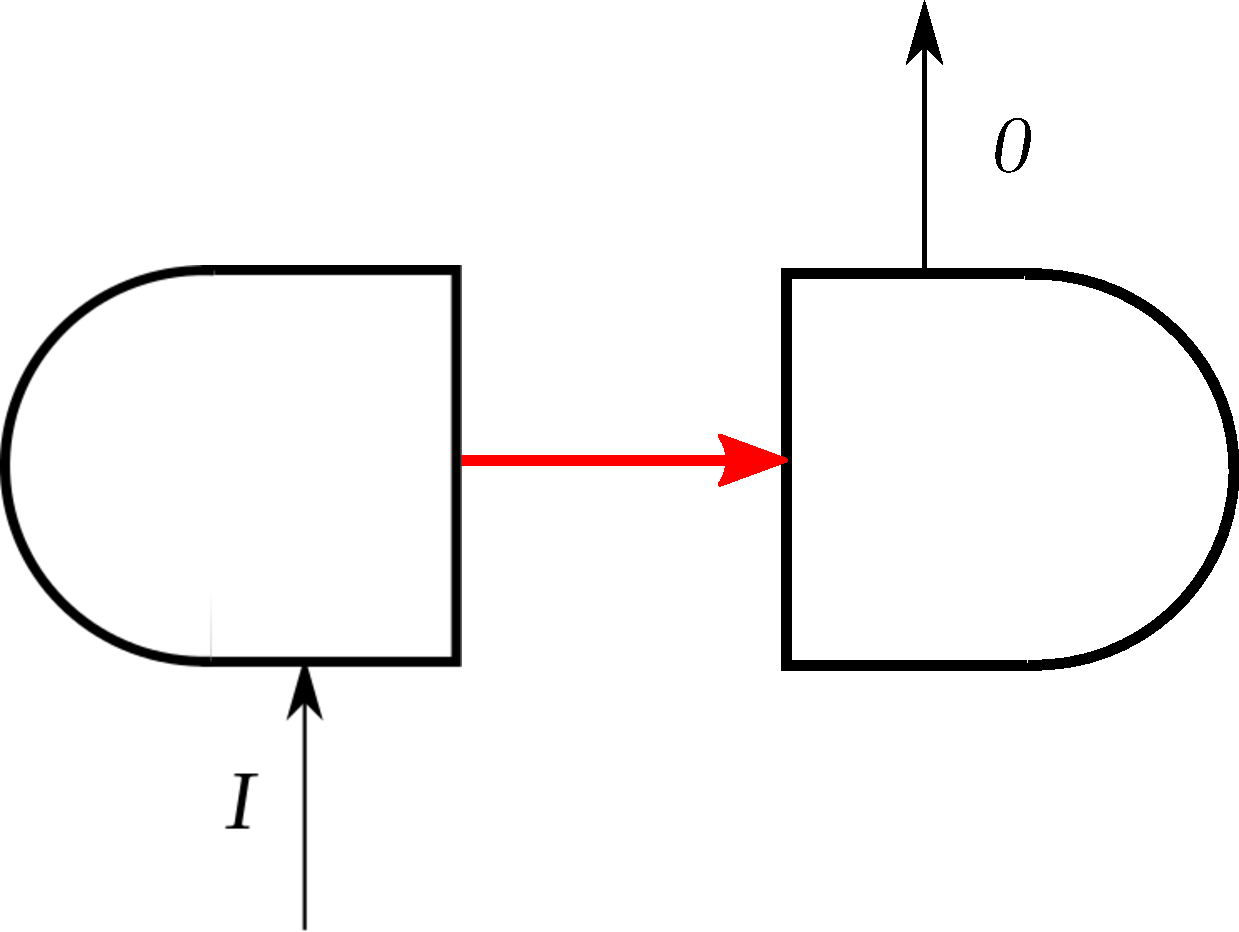
\includegraphics[width=2in]{quantum-proba.pdf}
\caption{ Probabilities are associated to a couple state-effect}
\label{ }
\end{center}
\end{figure}

General information processing quantum devices are constructed by building causal circuits out of these devices used as building blocks, thus constructing complicated apparatus out of simple ones.
An information theoretic formalism is obtained by choosing axioms on the properties of such devices (states and effects) and  operational rules to combine these devices and circuits and the associated probabilities, thus obtaining for  instance what is called in \cite{PhysRevA.84.012311} an operational probabilistic theory.
This kind of approach is usually considered for finite dimensional theories (which in the quantum case correspond to finite dimensional Hilbert spaces), both for mathematical convenience, and since this is the kind of system usually considered in quantum information science.

This approach  leads to a pictorial formulation of quantum information processing. It shares similarities with the ``quantum pictorialism" logic formalism, more based on category theory, and presented for instance in
\cite{Coecke-2010}.

It can also be viewed as an operational and informational extension of the convex set approach (developed notably by G. Ludwig, see
\cite{Ludwig:1985uq} and  \cite{Auletta},\cite{BeltCassi81} for details). This last approach puts more emphasis on the concept of states than on observables in QM.

I shall not discuss in any details these approaches. 
Let me just highlight amongst  the most recent attempts those of Hardy \cite{Hardy-2001,Hardy-2011} and those of Chiribella, D'Ariano \& Perinotti  
\cite{PhysRevA.81.062348, PhysRevA.84.012311} (
see \cite{Physics.4.55} for a short presentation of this last formulation).
See also \cite{MasMue2011}.
In \cite{PhysRevA.84.012311} the standard complex Hilbert space formalism of QM is derived from 6 informational principles: 
Causality,
Perfect Distinguishability,
Ideal Compression,
Local Distinguishability,
Pure conditioning,
Purification principle.

The first 2 principles are not very different from the principles of other formulations (causality is defined in a standard sense, and distinguishability is related to the concept of differentiating states by measurements).
The third one is related to existence of reversible maximally efficient compression schemes for states. 
The four and the fifth are about the properties of bipartite states and for instance the possibility to performing local tomography and the effect of separate atomic measurements on such states.
The last one, about ``purification'' distinguishes quantum mechanics from classical mechanics, and states that any mixed state of some system $\mathcal{S}$ may be obtained from a pure state of a composite larger system $\mathcal{S}+\mathcal{S}'$.
See \cite{Physics.4.55} for a discussion of the relation of this last purification principle with the discussions of the ``cut'' between the system measured and the measurement device done for instance by Heisenberg in \cite{pittphilsci8590}, but see of course the previous discussion by von Neumann in \cite{vonNeumann32G}.

\section{Quantum correlations}
\label{sQuCor}
The world of quantum correlations is richer, more subtle and more interesting than the world of classical ones. Most of the puzzling features and seeming paradoxes of quantum physics come from these correlations, and in particular from the phenomenon of entanglement. 
Entanglement is probably \emph{the} distinctive feature of quantum mechanics, and is a consequence of the superposition principle when considering quantum states for composite systems. Here I discuss briefly some basic aspects.
Entanglement describes the particular quantum correlations between two quantum systems which (for instance after some interactions) are in a non separable pure state,  so that each of them considered separately, is not in a pure state any more.
Without going into history, let me remind that if the terminology ``entanglement'' (``Verschr\"{a}nkung'') was introduced in the quantum context  by E. Schr\"{o}dinger in 1935 (when discussing the famous EPR paper).
However the mathematical concept 
%(the particular quantum correlations between two quantum systems which have interacted so that each of them considered separately  is not in a separable pure state any more)
 is older and goes back to the modern formulation of quantum mechanics. 
 For instance, some peculiar features of entanglement and its consequences have been  discussed already around the 30' in relation with the theory of quantum measurement by Heisenberg, von Neumann, Mott, etc. Examples of interesting entangled many particles states are provided by the Stater determinant for many fermion states, by the famous Bethe ansatz for the ground state of the spin 1/2 chain, etc.
 
\subsection{Entropic inequalities}
\paragraph{von Neumann entropy:} The difference between classical and quantum correlations is already visible when considering the properties of the von Neumann entropy of states of composite systems.
Remember that the von Neumann entropy of a mixed state of a system $A$, given by a density matrix $\rho_A$, is given by
\index{von Neumann entropy}
\begin{equation}
\label{ }
S(\rho_A)=-\tr(\rho_A\log\rho_A)
%S(\rho_A)=-\tr(\rho_A\ln\rho_A)
\end{equation}
In quantum statistical physics, the $\log$ is usually the natural logarithm
\begin{equation}
\label{ }
\log=\log_{\emath}=\ln
\end{equation}
while in quantum information, the $\log$ is taken to be the binary logarithm
\begin{equation}
\label{ }
\log=\log_{2}
\end{equation}
The entropy measures the amount of ``lack of information" that we have on the state of the system.  But in quantum physics, at variance with classical physics, one must be very careful about the meaning of ``lack of information'', since one cannot speak about the precise state of a system before making measurements. 
So the entropy could (and should) rather be viewed as a measure of the number of independent measurements we can make on the system before having extracted all the information, i.e. the amount of information we can extract of the system. It can be shown also that the entropy give the maximum information capacity of a quantum channel that we can build out of the system.
See \cite{Nielsen:2010fk} for a good introduction to quantum information and in particular on entropy viewed from the information theory point of view.

When no ambiguity exists on the state $\rho_A$ of the system $A$, I shall use the notations
\begin{equation}
\label{ }
S_A=S(A)=S(\rho_A)
\end{equation}

The von Neumann entropy shares many  properties of the classical entropy. It has the same  convexity properties
\begin{equation}
\label{ }
S[\lambda\rho+(1-\lambda)\rho']\ge \lambda S[\rho]+(1-\lambda)S[\rho']\quad,\qquad  0\le\lambda\le 1
\end{equation}
It is minimal $S=0$ for systems in a  pure state and maximal for systems in a equipartition state $S=\log(N)$ if $\rho={1\over N} \mathbf{1}_N$.
It is extensive for systems in separate states.

\paragraph{Relative entropy:} 
\index{Relative entropy}
The relative entropy (of a state $\rho$ w.r.t. another state $\sigma$ for the same system) is defined as in classical statistics (Kullback-Leibler entropy) as 
\begin{equation}
\label{ }
S(\rho\|\sigma)=\tr(\rho\log\rho)-\tr(\rho\log\sigma)
\end{equation}
with the same convexity properties.

The differences with the classical entropy arise for composite systems. For such a system $AB$, composed of two subsystems $A$ and $B$, a general mixed state is given by a density matrix $\rho_{AB}$ on $\mathcal{H}_{AB}=\mathcal{H}_{A}\otimes\mathcal{H}_{B}$.
The reduced density matrices for $A$ and $B$ are 
\begin{equation}
\label{ }
\rho_A=\tr_B(\rho_{AB})
\quad,\qquad
\rho_B=\tr_A(\rho_{AB})
\end{equation}
This corresponds to the notion of marginal distribution w.r.t. $A$ and $B$ of the general probability distribution of states for $AB$ in classical statistics.
Now if one considers
\begin{equation}
\label{ }
S({AB})=-\tr(\rho_{AB}\log\rho_{AB}),\quad
S({A})=-\tr(\rho_{A}\log\rho_{A}),\quad
S({B})=-\tr(\rho_{B}\log\rho_{B})
\end{equation}
one has the following definitions.
\paragraph{Conditional entropy:} 
\index{Conditional entropy} 
The \emph{conditional entropy} S(A|B) (the entropy of $A$ conditional to $B$ in the composite system $AB$) is
\begin{equation}
\label{ }
S(A|B)=S(AB) - S(B)
\end{equation}
The conditional entropy $S(A|B)$ corresponds to the remaining uncertainty (lack of information) on $A$ if $B$ is known.
\paragraph{Mutual information:} 
\index{Mutual information}
The \emph{mutual information} (shared by $A$ and $B$ in the composite system $AB$)
\begin{equation}
\label{MutInf}
S(A:B)=S(A)+S(B)-S(AB)
\end{equation}
\paragraph{Subadditivity:} 
\index{Subadditivity}
The entropy satisfies the general inequalities (triangular inequalities)
\begin{equation}
\label{subaddS}
|S(A)-S(B)|\le S({AB})\le S(A)+S(B)
\end{equation}
The rightmost inequality $S({AB})\le S(A)+S(B)$ is already valid for classical systems, but the leftmost  is quantum.
Indeed for classical systems the classical entropy $H_\mathrm{cl}$ satisfy only the much stronger lower bound
\begin{equation}
\label{CaddS}
\max(H_\mathrm{cl}(A),H_\mathrm{cl}(B)) \le H_\mathrm{cl}(AB)%\le S(A)+S(B)
\end{equation}

Subadditivity implies that if $AB$ is in a pure entangled state, $S(A)=S(B)$.
It also implies that the mutual information in a bipartite system is always positive
\begin{equation}
\label{MutInfPos}
S(A:B)\ge 0
\end{equation}

In the classical case the conditional entropy is always positive $H_\mathrm{cl}(A|B)\ge 0$.
In the quantum case the conditional entropy may be negative $S(A|B)< 0$ if the entanglement between $A$ and $B$ is large enough.
%This is different from the classical situation where the conditional entropy corresponds to the remaining uncertainty (lack of information) on $A$ if $B$ is known and is always $>0$.
This is a crucial feature of quantum mechanics. If $S(A|B)<0$ it means that $A$ and $B$ share information resources (through entanglement) which get lost if one gets information on $B$ only (through a measurement on $B$ for instance). 

\paragraph{Strong subadditivity:}
\index{Strong subadditivity}
Let us consider a tripartite systems $ABC$. The entropy satisfies another very interesting inequality
\begin{equation}
\label{StrSubAdd1}
S(A)+S(B)\le S({AC})+S({BC})
\end{equation}
It is equivalent to (this is the usual form)
\begin{equation}
\label{StrSubAdd2}
S({ABC})+S({C})\le S({AC})+S({BC})
\end{equation}
Note that \ref{StrSubAdd1} is also true for the classical entropy, but then for simple reasons. In the quantum case it is a non trivial inequality.


The strong subadditivity inequality implies the triangle inequality for tripartite systems
\begin{equation}
\label{ }
S(AC)\le S(AB)+S(BC)
\end{equation}
so the entropic inequalities can be represented graphically as in fig.~\ref{fSSubT}
\begin{figure}[h]
\begin{center}
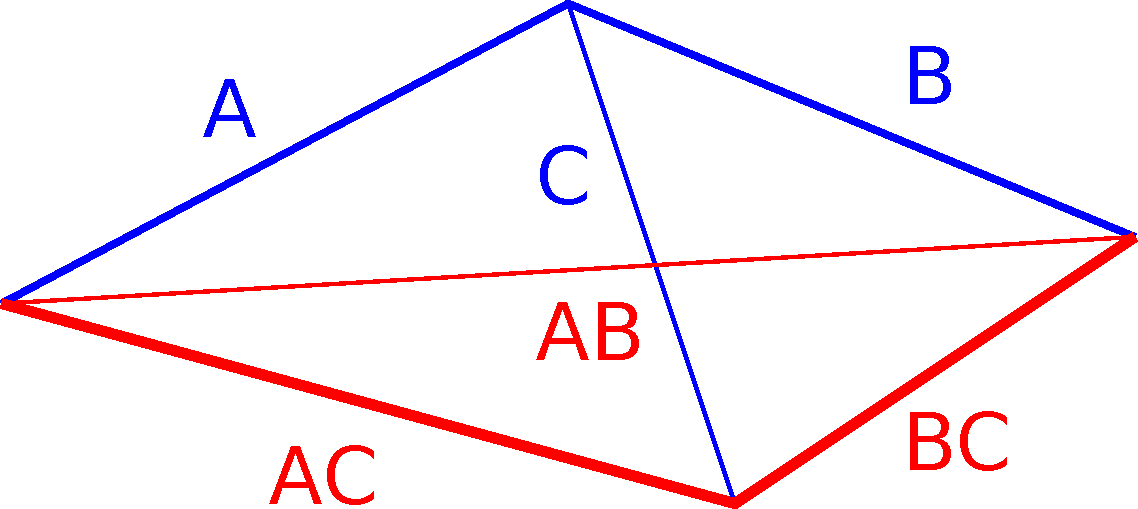
\includegraphics[width=2in]{Entropic-tetraedron.pdf}
\caption{Entropic inequalities: the length of the line ``$X$''  is the von Neumann entropy $S(X)$. The tetrahedron has to be ``oblate", the sum {\color{red}{AC+BC}} (fat red lines) is always $\ge$ the sum {\color{blue}{A+B}} (fat blue lines). }
\label{fSSubT}
\end{center}
\end{figure}

The strong subadditivity inequality has important consequences for conditional entropy and mutual information (see \cite{Nielsen:2010fk}). 
Consider a tripartite composite system $ABC$.
It implies for instance 
\begin{equation}
\label{ }
S(C|A)+S(C|B) \ge 0
\end{equation}
and
\begin{equation}
\label{ }
S(A|BC)\le S(A|B) 
\end{equation}
which means that conditioning A to a part of the external subsystem (here C inside BC) increase the information we have on the system (here A).
One has also for the mutual information
\begin{equation}
\label{ }
S(A:B)\le S(A:BC) 
\end{equation}
This means that discarding a part of a multipartite quantum system (here $C$) increases the mutual information (here between $A$ and the rest of the system).
This last inequality is very important. It implies for instance that if one has a composite system $AB$, performing some quantum operation on $B$ without touching to $A$ cannot increase the mutual information between $A$ and the rest of the system. 

%This is related to the fact that one cannot transmit information in an  acausal way between two part of a bipartite system in an entangled state (EPR-like experiment). 
%In other words, quantum mechanics allows some non-local correlations, but no action-at-a-distance is allowed (non-signalling).
%\emph{CHECK!}
Let us mention other subadditivity inequalities for tri- or quadri-partite systems.
%\begin{equation}
%\label{ }
%S(AB|CD)\le S(A|C) + S(B|D)
%\end{equation}
%\begin{equation}
%\label{ }
%S(AB|C)\le S(A|C) + S(B|C)
%\end{equation}
%\begin{equation}
%\label{ }
%S(A|BC)\le S(A|B) + S(A|C)
%\end{equation}
\begin{align}
\label{ }
S(AB|CD)&\le S(A|C) + S(B|D)
\\
\label{ }
S(AB|C)&\le S(A|C) + S(B|C)
\\
\label{ }
S(A|BC)&\le S(A|B) + S(A|C)
\end{align}


%\hrule
%
%\begin{equation}
%\label{ }
%|S_A-S_B|\le S_{AB}\le S_A+S_B
%\end{equation}
%
%
%
%
%\begin{equation}
%\label{ }
%S_A+S_B\le S_{AC}+S_{BC}
%\end{equation}
%
%\begin{equation}
%\label{ }
%S_{ABC}+S_{C}\le S_{AC}+S_{BC}
%\end{equation}
%
%Relative entropy (of a state $\rho$ w.r.t. another state $\sigma$ for the same system)
%\begin{equation}
%\label{ }
%S(\rho\|\sigma)=\tr(\rho\log\rho)-\tr(\rho\log\sigma)
%\end{equation}
%Conditional entropy (of $A$ w.r.t. $B$ in composite system $AB$)
%\begin{equation}
%\label{ }
%S(A|B)=S(AB) - S(B)
%\end{equation}
%Mutual information (of $A$ and $B$ in composite system $AB$)
%\begin{equation}
%\label{ }
%S(A:B)=S(A)+S(B)-S(AB)
%\end{equation}

\subsection{Bipartite correlations:}
The specific properties of quantum correlations between two causally separated systems are known to disagree with
%lead to strong violations of 
what one would expect from a ``classical picture'' of quantum theory, where the quantum probabilistics features come just from some lack of knowledge of underlying ``elements of reality''.
I shall come back later on the very serious problems with the ``hidden variables'' formulations of quantum mechanics.
But let us discuss already some of the properties of these quantum correlations in the simple case of a bipartite system. 

I shall discuss briefly one famous and important result: the  Tsirelson bound.
The general context is that of the discussion of non-locality issues and of Bell's \cite{Bell:1964kc} and CHSH inequalities \cite{PhysRevLett.23.880} in bipartite systems. 
However, since these last inequalities are more of relevance when discussing hidden variables models, I postpone their discussion to
the next section \ref{sHidVar}.

This presentation is standard and simply taken from \cite{Laloe-book}.



\subsubsection{The Tsirelson Bound}
\label{ssTsiBn}
\index{Tsirelson bound}

\paragraph{The two spin system:} Consider a simple bipartite system consisting of two spins 1/2, or q-bits 1 and 2.
If two observers (Alice $\mathcal{A}$ and Bob $\mathcal{B}$) make independent measurements of respectively the value of the spin 1 along some direction $\vec n_1$ (a unit vector in 3D space)
and of the spin 2 along $\vec n_2$, at each measurement they get results (with a correct normalization) $+1$ or $-1$.
Now let us compare the results of four experiments, depending whether $\mathcal{A}$ choose to measure the spin 1 along a first direction $\vec a$ or a second direction $\vec a'$, and wether $\mathcal{B}$ chose (independently) to measure the spin 2 along a first direction $\vec b$ or a second direction $\vec b'$. Let us call the corresponding observables $\mathbf{A}$, $\mathbf{A'}$, $\mathbf{B}$, $\mathbf{B'}$, and by extension the results of the corresponding measurements in a single experiment $A$ and $A'$ for the first  spin, $B$ and $B'$ for the second spin.
%$$2 \vec S_1{\cdot}\vec n$$

\begin{equation}
\label{ }
\text{spin 1 along }\ \vec a \quad \to\quad A= \pm 1
\quad;\quad
\text{spin 1 along }\ \vec a' \quad \to\quad A'= \pm 1
\end{equation}

\begin{equation}
\label{ }
\text{spin 2 along }\ \vec b \quad \to\quad B= \pm 1
\quad;\quad
\text{spin 2 along }\ \vec b' \quad \to\quad B'= \pm 1
\end{equation}

Now consider the following combination $M$ of products of observables, hence of products of results of experiments
\begin{equation}
\label{McorBHSH}
M=AB-A B' + A' B + A' B'
\end{equation}
and consider the expectation value $\langle M\rangle_\psi$ of $M$ for a given quantum state $|\psi\rangle$ of the two spins system.
In practice this means that we prepare the spins in state  $|\psi\rangle$, chose randomly (with equal probabilities) one of the four observables, and to test locality $\mathcal{A}$ and $\mathcal{B}$ may be causally deconnected, and choose independently (with equal probabilities) one of their own two observables, i.e. spin directions. Then they make their measurements. The experiment is repeated a large number of time  and the right average combination $M$ of the results of the measurements is calculated afterwards.

A simple explicit calculation shows the following inequality, known as the Tsirelson bound \cite{springerlink:10.1007/BF00417500}

\paragraph{Tsirelson bound:}
For any state and any choice orientations $\vec a$, $\vec a'$, $\vec b$ and $\vec b'$, one has
\begin{equation}
\label{TsirBound}
|\langle M\rangle |\le 2\sqrt{2}
\end{equation}
while, as discussed later, ``classically'', i.e. for theories where the correlations are described by contextually-local hidden variables attached to each subsystem, one has the famous Bell-CHSH bound \index{CHSH inequality}
\begin{equation}
\label{ }
\langle|M|\rangle_\mathrm{``classical''}\le 2.
\end{equation}
The Tsirelson bound is saturated if the state $|\psi\rangle$ for the two spin is the singlet
\begin{equation}
\label{ }
|\psi\rangle=|\text{singlet}\rangle={1\over \sqrt{2}}\left(  |\uparrow\rangle\otimes | \downarrow\rangle - |\downarrow\rangle\otimes | \uparrow\rangle \right)
\end{equation}
and the directions for  $\vec a$, $\vec a'$, $\vec b$ and $\vec b'$ are coplanar, and such that $\vec a\perp\vec a'$, $\vec b\perp\vec b'$, and the angle between $\vec a$ and $\vec b$ is $\pi/4$, as depicted on \ref{figBCHSH}.
\begin{figure}[h]
\begin{center}
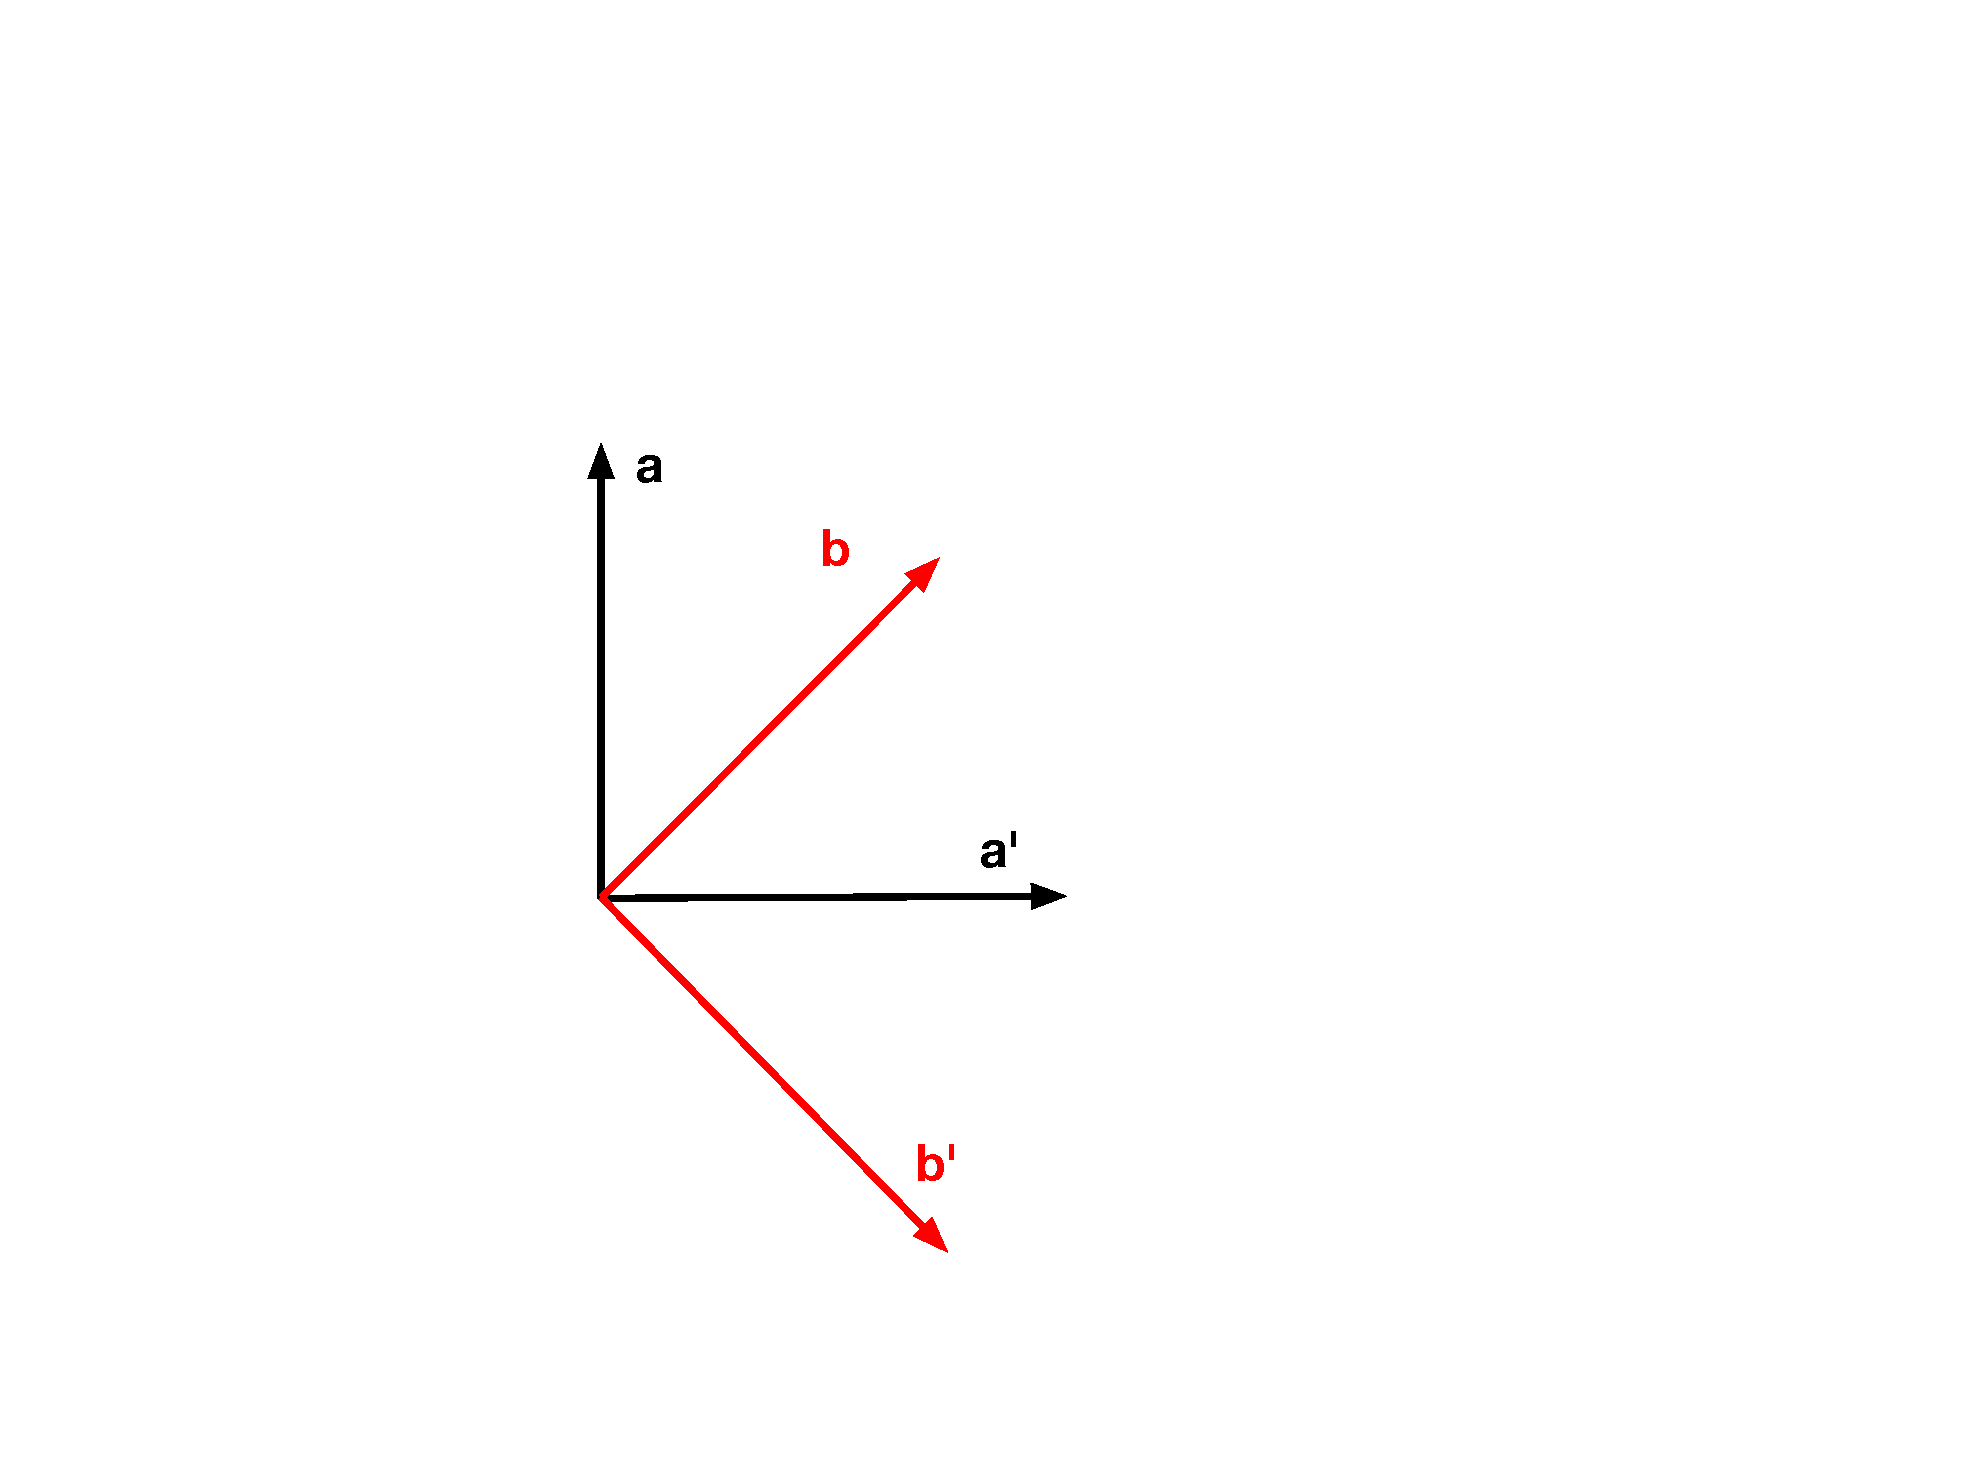
\includegraphics[width=1.8in]{Bchsh.pdf}
\caption{Spin directions for saturating the Tsirelson bound and maximal violation of the Bell-CHSH inequality}
\label{figBCHSH}
\end{center}
\end{figure}

\subsubsection{Popescu-Rohrlich boxes}
\index{Popescu-Rohrlich boxes}
\paragraph{Beyond the Tsirelson bound ?}
Interesting questions arise when one consider what could happen if there are ``super-strong correlations'' between the two spins (or in general between two subsystems) that violate the Tsirelson bound.
Indeed, the only mathematical bound on $M$ for general correlations is obviously $|\langle M\rangle|\le 4$.
Such hypothetical systems are considers in the theory of quantum information and are denoted Popescu-Rohrlich boxes
\cite{springerlink:10.1007/BF02058098}
. 
With the notations of the previously considered 2 spin system, BR-boxes consist in a collection of probabilities $P(A,B|a,b)$
for the outputs $A$ and $B$ of the two subsystems, the input or settings $a$ and $b$ being fixed. 
The $(a,b)$ correspond to the settings $I$ and the $(A,B)$ to the outputs $O$ of fig.~\ref{fdevice} of the quantum information section.
In our case we can take for the first spin
\begin{equation}
\label{ }
a=1\ \to\ \text{chose orientation}\  \vec a\quad,\qquad
a=-1\ \to\ \text{chose orientation}\  \vec a'
\end{equation}
and for the second spin
\begin{equation}
\label{ }
b=1\ \to\ \text{chose orientation}\  \vec b\quad,\qquad
b=-1\ \to\ \text{chose orientation}\  \vec b'
\end{equation}
The possible outputs being always $A=\pm 1$ and $B=\pm 1$.


\begin{figure}[h]
\begin{center}
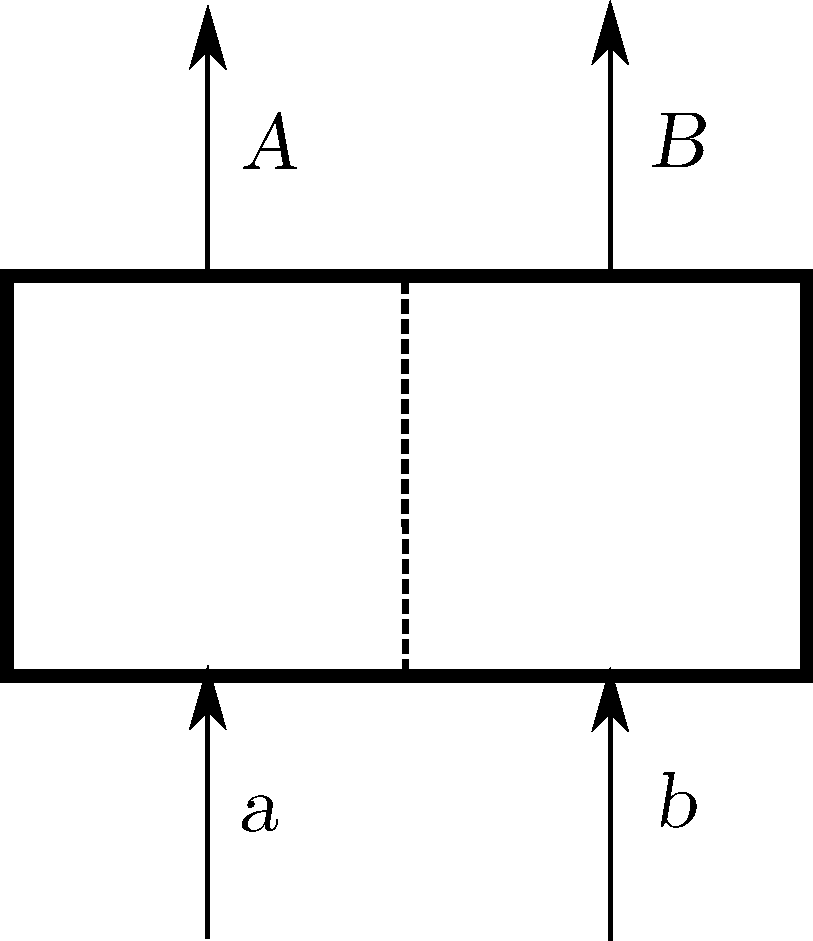
\includegraphics[width=2in]{PR-box.pdf}
\caption{a Popescu-Rohrlich box}
\label{fPRbox}
\end{center}
\end{figure}

The fact that the $P(A,B|a,b)$ are probabilities means that
\begin{equation}
\label{ }
0\le P(A,B|a,b)\le 1\quad,\qquad \sum_{A,B}P(A,B|a,b)=1\quad\text{for}\quad a,b\ \text{fixed}
\end{equation}
\paragraph{Non signalling:} 
If the settings $a$ and $b$ and the outputs $A$ and $B$ are relative to two causally separated parts of the system, corresponding to manipulations by two independent agents (Alice and Bob), enforcing causality means that Bob cannot guess which setting ($a$ or $a'$) Alice has chosen from his choice of setting ($b$ and $b'$) and his output ($B$ or $B$), without knowing Alices' output $A$. The same holds for Alice with respect to Bob.
This requirement is enforced by the non-signaling conditions
\begin{align}
\label{}
    \sum_A P(A,B|a,b) = &  \sum_A P(A,B|a',b) \\
    \sum_B P(A,B|a,b) = &  \sum_B P(A,B|a,b')  
\end{align}

A remarkable fact is that there are choices of probabilities which respect the non-signaling condition (hence causality) but violate the Tsirelson  bound and even saturate the absolute bound $|\langle M\rangle|=4$ .
Such hypothetical devices  would allow to use ``super-strong correlations'' (also dubbed ``super-quantum correlations'') to manipulate and transmit information in a more efficient way that quantum systems (in the standard way of quantum information protocols, by sharing some initially prepared bipartite quantum system and exchanges of classical information) 
\cite{PhysRevLett.96.250401}
\cite{vanDam2005}
\cite{10.1038/nature08400}
.  However, besides these very intriguing features of ``trivial communication complexity", such devices are problematic. 
For instance it seems that no interesting dynamics can be defined on such systems  \cite{PhysRevLett.104.080402}.


\section{The problems with hidden variables}
\label{sHidVar}
%\subsection{The idea}
\subsection{Hidden variables and ``elements of reality''}
\index{Hidden variable}
In this section I discuss briefly some features of quantum correlations which are important when discussing the possibility that the quantum probabilities may still have, to some extent, a ``classical interpretation'' by reflecting our ignorance of inaccessible ``sub-quantum'' degrees of freedom or ``elements of reality'' of quantum systems, which could behave in a more classical and deterministic way. In particular a question is: which general  constraints on such degrees of freedom are enforced by quantum mechanics?

This is the general idea of the ``hidden variables'' program and of the search of explicit hidden variable models. These ideas go back to the birth of quantum mechanics, and were for instance proposed by L. de Broglie in his first ``pilot wave model'', but they were abandoned by most physicist after 1927 Solvay Congress and the advances of the 1930' , before experiencing some revival  and setbacks in the 1960', from the works by Bohm and de Broglie, and the discussions about locality and Bell-like inequalities.

The basic idea is that when considering a quantum system $\mathcal{S}$, its state could be described by some (partially or totally) hidden variables $\mathfrak{v}$ in some space $\mathfrak{V}$, with some unknown statistics and dynamics. 
Each $\mathfrak{v}$ may represent a (possibly infinite) collection of more fundamental variables.
But they are such that the outcome of a measurement operation of a physically accessible  observables $A$ is  determined by the hidden variable $\mathfrak{v}$. \begin{equation}
\label{m2oVD}
\text{mesurement of}\quad A\ \to \ \text{outcome}\quad a=f(A,\frak{v})\quad\text{(a real number)}
\end{equation}
Quantum undeterminism should come from our lack of knowledge on the exact state of the hidden variables.
In other word, the pure quantum states $|\psi\rangle$ of the system should correspond to some classical probability distribution $p_\psi(\mathfrak{v})$ on $\mathcal{V}$.
Of course a measurement operation could back react on the hidden variables $\mathfrak{v}$.

This is probably an oversimplified presentation of the idea, since there are several versions and models. But for instance in the hidden variable model of de Broglie and Bohm (for a single particle obeying the Schr\"{o}dinger equation), the hidden variable $\mathfrak{v}=(\psi,x)$, where $\psi=\{\psi(y)\}$ is the whole ``pilot" wave function, and $x$ the position of the particle.

In its simplest version, one could try to consider hidden variables (element of reality) that are in one to one correspondence with the possible outcomes $a$ of all the observables $A$ of the system, and in particular which obeys the addition law
\begin{equation}
\label{CHVvN}
C=A+B \quad\implies\quad c=a+b\quad\text{i.e}\qquad f(C,\frak{v})=f(A,\frak{v})+f(B,\frak{v})
\end{equation}
This possibility is already discussed by J. von Neumann in his 1932 book
\cite{vonNeumann32G,vonNeumann32}, 
\index{von Neumann J.}
where it is shown to be clearly inconsistent. Indeed if $A$ and $B$ do not commute, the possible outcomes of $C$ (the eigenvalues of the operator $C$) are not in general sums of outcomes of $A$ and $B$ (sums of eigenvalues of $A$ and $B$), since $A$ and $B$ do not have common eigenvectors.
See \cite{Bub:2010kx} for a detailed discussion of the argument and of its historical significance.

%\section{Reality, contextuality and non-locality}
%\subsection{The von-Neumann argument}

\subsection{Context free hidden variables ?}
\index{Noncontextuality}
Hidden variable models have been rediscussed a few decades later, from a more realistic point of view, in particular by J. Bell.
In a modern language, the models considered are  ``context free'' or ``non contextual''  hidden variables models. 
The idea is that one should consider only the correlations between results of  measurements  on a given system for \emph{sets of commuting observables}. Indeed only such measurements can be performed independently and in any possible order (on a single realization of the system), and without changing the statistics of the outcomes. Any such given set  of observables can be thought as a set of classical observables, but of course this classical picture is not consistent from one set to another.

Thus the idea is still that a hidden variable $\mathfrak{v}$ assigns to any observable $A$ an outcome $a=f(A,\mathfrak{v})$ as in \ref{m2oVD}.
This assumption is often called ``value definiteness'' (VD).
\index{Value definiteness} 

However the very strong constraint \ref{CHVvN} should be replaced by the more realistic constraint for the set of outcomes $\{f(A,\mathfrak{v})$

\begin{align}
\label{CHVNCon}
\text{if $A$ and $B$ commute, then}\quad\begin{cases}
      & f(A+B,\mathfrak{v})=f(A,\mathfrak{v})+f(B,\mathfrak{v})\\
      &\hskip 5em \text{and} \\
      & f(AB,\mathfrak{v})=f(A,\mathfrak{v})f(B,\mathfrak{v})
\end{cases}
\end{align}
Moreover, these conditions are extended to  any  family $\mathcal{F}=\{A_i,\,i=1,2,\cdots\}$ of commuting operators.

Here I consider purely deterministic HV. This means that the assignement  $A\to a=f(A,\frak{v})$ is unique, and thus in QM $a$ is one of the eigenvalues of the operator $A$. 

The term ``context free'' means that the outcome $a$ for the measurement of the first  observable $A$  is supposed to be independent of the choice of the second observable  $B$. 
In other word, the outcome of a measurement depends on the hidden variable, but not of the ``context'' of the measurement, that is of the other  quantities measured at the same time.

We shall discuss the possibility that $a$ is a random variable (with a law fixed by $\mathfrak{v}$) later.

\subsection{Gleason's theorem and contextuality}
\label{ssGTCont}
\index{Gleason's theorem}
\index{Contextuality}
These kind of models seem much more realistic. 
However, they are immediatly excluded by  Gleason's theorem \cite{Gleason57}, as already argued by J. Bell in \cite{RevModPhys.38.447}.

Indeed, if to any $\mathfrak{v}$ is associated a function $f_\mathfrak{v}$, defined as
\begin{equation}
\label{ }
f_\mathfrak{v}\quad;\qquad A\to f_\mathfrak{v}(A)=f(A,\mathfrak{v})
\end{equation}
which satisfy  the consistency conditions \ref{CHVNCon}, this is true in particular for any family of commuting projectors $\{P_i\}$, whose outcome in $0$ or $1$
\begin{equation}
\label{ }
P\ \text{projector such that}\ \ P=P^\dagger=P^2\quad\implies\quad f_\mathfrak{v}(P)=0\ \text{or}\ 1
\end{equation}
In particular, this is true for the family of projectors $\{P_i\}$ onto the vector of any orthonormal basis $\{\vec e_i\}$ of the Hilbert space $\mathcal{H}$ of the system. This means simply that defining the function $f$ on the unit vectors $\vec e$ by 
\begin{equation}
\label{eNCdef}
f(\vec e)=f_\mathfrak{v}(P_{\vec e})\quad,\qquad P_{\vec e}=|\vec e\rangle\langle \vec e|
\end{equation}
(remember that $\mathfrak{v}$ is considered fixed), this function must satisfy for any orthonormal basis 
\begin{equation}
\label{eNCframe}
\{\vec e_i\}\quad\text{orthonormal basis}\qquad\implies\qquad \sum_i f(\vec e_i)=1
\end{equation}
while we have for any unit vector
\begin{equation}
\label{eNCproj}
f(\vec e)\ =\ 0\ \text{or}\ 1
\end{equation}
This contradicts strongly Gleason's theorem (see \ref{ssGleason}), as soon as the Hilbert space of the system $\mathcal{H}$ has dimension $\text{dim}(\mathcal{H}) \ge 3$! 
Indeed, \ref{eNCframe} means that the function $f$ is a frame function (in the sense of Gleason), hence is continuous, while $\ref{eNCproj}$ (following from the fact that $f$ is function on the projectors) means that $f$ cannot be a continuous function. So
\begin{equation}
\label{ }
\text{dim}(\mathcal{H}) \ge 3\implies\text{no context-free HV can describe  all the quantum correlations}
\end{equation}
Gleason's theorem is a very serious blow to the HV idea. However, some remaining possibilities can be considered, for instance:
\begin{enumerate}
 \item There are still context-free HV, but they describe only some specific subset of the quantum correlations, not all of them.
  \item There are HV, but they are fully contextual.
\end{enumerate} 
We now discuss two famous cases where the first  option has been explored, but appears to be still problematic.
The second one raises also big questions, that will be shortly discussed in \ref{ssHVdisc}.
 
\subsection{The Kochen-Specker theorem}
\index{Kochen-Specker theorem}
The first option is related to the idea that some subset of the correlations of a quantum system have a special status, being related to some special explicit ``elements of reality'' (the ``be-ables'' in the terminology of J. Bell), by contrast to the ordinary observables which are just ``observ-ables''. Thus a question is whether for a given quantum system there are  finite families of non commuting observables which can be associated to context-free HV.

In fact the problems with non-contextual HV have been shown to arise already for very small such subsets of observables, first by S. Kochen and E. Specker \cite{KochenSpecker67}. These issues started to be discussed by J. Bell in
\cite{RevModPhys.38.447}. 
This is the content of the  Kochen-Specker theorem. This theorem provides in fact examples of finite families of unit vectors $\mathcal{E}=\{\vec e_i\}$ in a Hilbert Space $\mathcal{H}$ (over $\mathbb{R}$ or $\mathbb{C}$) of finite dimension ($\mathrm{dim}(\mathcal{H})=n$), such that it is impossible to find any  frame function such that
\begin{equation}
\label{ }
f(\vec e_i)=0\ \text{or}\ 1
\quad\text{and}\quad
(\vec e_{i_1},\cdots, \vec  e_{i_n})\quad\text{orthonormal basis}\quad\implies\quad \sum_{a=1}^n f(\vec e_{i_a})=1
\end{equation}
The original example of \cite{KochenSpecker67} involved a set with 117 projectors in a 3 dimensional Hilbert space and is a very nice example of non-trivial geometry calculation.  Simpler examples in dimension $n=3$ and $n=4$ with less projectors have been provided  by several authors (Mermin, Babello, Peres, Penrose).

I do not discuss more these examples and their significance. But this shows that the non--contextual character of quantum correlations is a fundamental feature of quantum mechanics.

\subsection{Bell / CHSH inequalities and non-locality}
Another important situation where non-contextuality is explored, in relation with locality, is found in the famous 1964 paper by J. Bell 
\cite{Bell:1964kc}. 
\index{Bell inequality}
\index{CHSH inequality}
Consider a bipartite system $\mathcal{S}$ consisting of two causally separated subsystems $\mathcal{S}_1$ and $\mathcal{S}_2$, for instance a pair of time-like separated photons in a  Bell-like experiment. One is interested in the correlations between the measurements that are performed independently on $\mathcal{S}_1$ and $\mathcal{S}_2$. 
Any pair of corresponding observables $A$ and $B$ (or more exactly $A\otimes 1$ and $1\otimes B$) commute, and thus one expect that the result of a measurement on $\mathcal{S}_1$, if it depends on some HV, should not depend on the measurement made on $\mathcal{S}_2$. In other word, the result of a measurement on $\mathcal{S}_1$ should not depend on the context of $\mathcal{S}_2$. The reciprocal statement being true as well. 

Thus, following Bell, let us assume that some HV's underlie the bipartite system $\mathcal{S}$, and that it is local in the sense that it is $\mathcal{S}_1$-versus-$\mathcal{S}_2$ context free. But it may not -- and in fact  it cannot -- be context-free with respect to $\mathcal{S}_1$ or $\mathcal{S}_2$ only. This means that a given HV $\mathfrak{v}$ should determine separately the relation \emph{observable $A\to$ outcome $a$}  for  $\mathcal{S}_1$  and  \emph{observable $B\to$ outcome $b$} for $\mathcal{S}_2$. In other word, such a hidden variable assigns a pair of probability distributions for all the observables relative to $\mathcal{S}_1$ and $\mathcal{S}_2$
\begin{equation}
\label{locHV}
\mathfrak{v}\quad
\mapsto\quad (p_1(a|A),p_2(b|B))
\end{equation}
The function $p_1(a|A)$ give the probability for the outcome $a$ when measuring $A$ on $\mathcal{S}_1$, the function $p_1(a|A)$  the probability for the outcome $b$ when measuring $B$ on $\mathcal{S}_2$.

One may assume that these probabilities can be decomposed into subprobabilities associated to local hidden variables $\mathfrak{w}_1$ and $\mathfrak{w}_2$  for the two subsystems $\mathcal{S}_1$ and $\mathcal{S}_2$. In this case $\mathfrak{v}$ is itself a pair of probability distribution $(q_1,q_2)$ over the $\mathfrak{w}_1$'s and $\mathfrak{w}_2$'s respectively.
\begin{equation}
\label{ }
\mathfrak{v}=(q_1,q_2)
\quad,\qquad q_1:\ \mathfrak{w}_1\to q_1(\mathfrak{w}_1)\ ,\ \ q_2:\ \mathfrak{w}_2\to q_1(\mathfrak{w}_2)
\end{equation} 
while it is the HV $\mathfrak{w}_1$ (respectively $\mathfrak{w}_2$) that determines the outcome $A\to a$ (respectively $B\to b$). 
These HV,s have to be contextual if one wants the relations $A\to a$ and $B\to b$  to be consistent with quantum mechanics for the two subsystems.

But one may also take the probability distributions $p_1(a|A)$ and $p_2(b|B)$ to be fully quantum mechanical, thus corresponding, using Gleason's theorem, to some density matrices $\rho_1$ and $\rho_2$ 
\begin{equation}
\label{ }
\mathfrak{v}=(\rho_1,\rho_2)
\end{equation} 
such that 
$p_1(a|A)=\tr(\delta(a-A)\rho_1)$ and $p_2(b|B)=\tr(\delta(b-B)\rho_2)$.

In any case,  hidden variables of the form \ref{locHV} are denoted ``local hidden variables''.
One might perhaps rather call them 
``locally-contextual-only hidden variables" 
but let us keep the standard denomination.

A quantum state $\psi$ of $\mathcal{S}$ corresponds to some probability distribution $q(\mathfrak{v})$ over the HV's $\mathfrak{v}$.
$q(\mathfrak{v})$ represent our ignorance about the ``elements of reality''  of the system.
If this description is correct, the probability for the pair of outcomes $(A,B)\to (a,b)$ in the state $\psi$ is given by the famous representation
\begin{equation}
\label{probABloc}
p(a,b|A,B)=\sum_{\mathfrak{v}} q(\mathfrak{v})\,p_1(a|A)\,p_2(b|B)
\end{equation}
It is this peculiar form which implies the famous Bell and BHSH inequalities on the correlations between observables on the two causally independent subsystems. Let us repeat the argument for the CHSH inequality.
If we consider for observables for $\mathcal{S}_1$ (respectively   $\mathcal{S}_2$) two (not necessarily commuting) projectors $P_1$ and $P'_1$ (respectively $Q_2$ and $Q'_2$), with outcome $0$ or $1$, and redefine them as
\begin{equation}
\label{ }
A=2 P_1-1\,\quad A'=2 P'_1-1\,\quad B=2 Q_1-1\,\quad B'=2 Q'_1-1\,\quad
\end{equation}
so that the outcomes are $-1$ or $1$,
if one perform a series of experiments on an ensemble of independently prepared instances of the bipartite system $\mathcal{S}$, choosing randomly with equal probabilities to measure $(A,B)$, $(A',B)$, $(A,B')$ or $(A',B')$, and combine the results to compute the average 
\begin{equation}
\label{ }
\langle M\rangle = \langle AB\rangle -\langle A B' \rangle +\langle  A' B\rangle  +\langle  A' B'\rangle 
\end{equation}
the same argument than in \ref{ssTsiBn}, using the general inequality
\begin{equation}
\label{ }
a,a',b,b'\in[-1,1] \quad\implies\quad a(b-b')+a'(b+b')\in[-2,2]
\end{equation}
implies the CSHS inequality
\begin{equation}
\label{CSHSineq}
-2\le \langle M\rangle\le  2
\end{equation}
\index{Bell inequality}
\index{CHSH inequality}
This inequality is known to be violated for some quantum states (entangled states) and some choice of observables. Indeed $\langle M\rangle$ may saturate the Tsirelon's bound $|\langle M\rangle |\le 2\sqrt{2}$.
\index{Tsirelson bound}
The reason is simple. Assuming that all quantum states give probabilities of the form  \ref{probABloc} and that the probabilities $p_1(a|A)$ and $p_2(b|B)$ obey the quantum rules and are representable by density matrices means that any quantum state (mixed or pure) $\psi $ can be represented by a density matrix of the form
\begin{equation}
\label{ }
\rho=\sum_{\mathfrak{v}} q(\mathfrak{v})\  \rho_1(\mathfrak{v}) \otimes \rho_2(\mathfrak{v})
\end{equation}
Such states are called separable states.
\index{Separable state}
\index{Non-locality}
But not all states are  separable. 
 For a bipartite system, 
this is the case indeed for pure  entangled states.

I do not discuss the many and very interesting generalizations and variants of Bell inequalities (for instance the spectacular GHZ example for tripartite systems) and the possible consequences and tests of non-contextuality.


I do not review either all the experimental tests of violations of Bell-like inequalities in various contexts, starting from the first experiments by Clauser, and those by Aspect et al., up to the most recent ones. They are in full agreement with the predictions of standard Quantum Mechanics and more precisely of Quantum Electro Dynamics. See for instance \cite{Laloe-book} or a recent and very complete review. 

\subsection{Discussion}
\label{ssHVdisc}
The significance and consequences of Bell and CHSH inequalitys and of the Kochen-Specker theorem have been enormously discussed, and some debates are still going on. To review and summarize these discussions is not the purpose of these notes. 
Let me just try to make some simple remarks.

The assumption of context-free value definiteness is clearly not tenable, from Gleason's theorem. This means that one must be very careful when discussing quantum physics about correlations between results of measurements. To quote a famous statement by Peres: ``Unperformed experiments have no results''  \cite{Peres78}.

Trying to assign some special ontological status to a (finite and in practice small) number of observables to avoid the consequence of the Kochen-Specker theorem may be envisioned, but raises other problems. 
For instance, if one wants to keep the main axioms of QM, and non-contextuality, by using a finite number of observables, one would expect the quantum logic formalism would lead to QM on a finite division ring (a Galois field), but it is known that this is not possible (see the discussion in \ref{sssRing}).
Note however that relaxing some basic physical assumptions like reversibility and unitarity has been considered for instance in \cite{tHooft2007}.

It is also clear that non-local quantum correlations are present in non-separable quantum states, highlighted by the violations of Bell's and CHSH-like inequalities (and their numerous and interesting variants). They represent some of the most non-classical and counter-intuitive features of quantum physics.
In connexion with the discussions of the ``EPR-paradox'', this non-local aspect of quantum physics has been often -- and is still sometimes --presented as  a contradiction between the principles of quantum mechanics and those of special relativity.
This is of course not the case.
These issues must be discussed in the framework of relativistic quantum field theory, where the basic objects are quantum fields, not (first quantized) particles (or classical fields).
See the section \ref{ssAQFTdsh}.
In this formalism a quantum state of a field is (some kind of) wave function over fields configurations over the entire space, and is intrinsically a non-local and non-separable object. 
The physical requirements of causality, and locality, implying no faster-than-light signaling (or any kind of real ``spooky-at-a-distance action''), are requirements on the observables, i.e. on the self-adjoint operators of the theory.

%The significance of the 
\index{Contextuality}
Finally, the option (2) at the end of \ref{ssGTCont} -- \textit{There are hidden variables but that they are fully contextual} -- is also very problematic and raises more questions than solutions (in my opinion). 
For instance, I would expect that even assuming non-contextual value definiteness, the sum and product relations \ref{CHVNCon} should still holds for commuting observables with fully non-degenerate spectrum. Then a problem of definiteness arises when considering a projector as a limit of such observables (in some sense the result of a measurement should depend not only on all the measurements you can perform, but on those you will not perform).
Another problem is that contextuality leads to consider that there are non-local hidden correlation between the system and the measurement apparatus before any measurement, which in some sense pushes the problem one rug further without really solving it.
Nevertheless, contextuality has been considered by several authors in connexion with some interpretations of quantum mechanics like the so called ``modal interpretations''. I am however unable to discuss this further.

\medskip
To summarize the discussions of these last two sections \ref{sQuCor} and \ref{sHidVar}: 
Contrary to classical physics, there is an irreducible quantum uncertainty in the description of any quantum system. Not all its physical observable can be characterized at the same time. This is of course the uncertainty principle.
Contrary to a simple reasoning, this does not mean that a quantum system is always more uncertain or ``fuzzy''  than a classical system. Indeed, the quantum correlations are stronger than the classical correlations, as exemplified by the quantum entropic inequalities \ref{subaddS} and 
\ref{StrSubAdd1}, and the Tsirelson bound \ref{TsirBound} compared to their classical analog, the entropic bound \ref{CaddS} and the B-CHSH inequality \ref{CSHSineq}.
This can be represented by the little drawing of Fig.~\ref{QYantra}.
This is why the results by J. Bell and the subsequent ones turned out to have a long term impact. They contributed to the realization of what is not quantum mechanics, and to the rise of quantum information: using quantum correlations and entanglement, it is possible to  transmit and manipulate information, perform calculations, etc.  in ways which are impossible by classical means, and which are much more efficient.

\begin{figure}[h]
\begin{center}
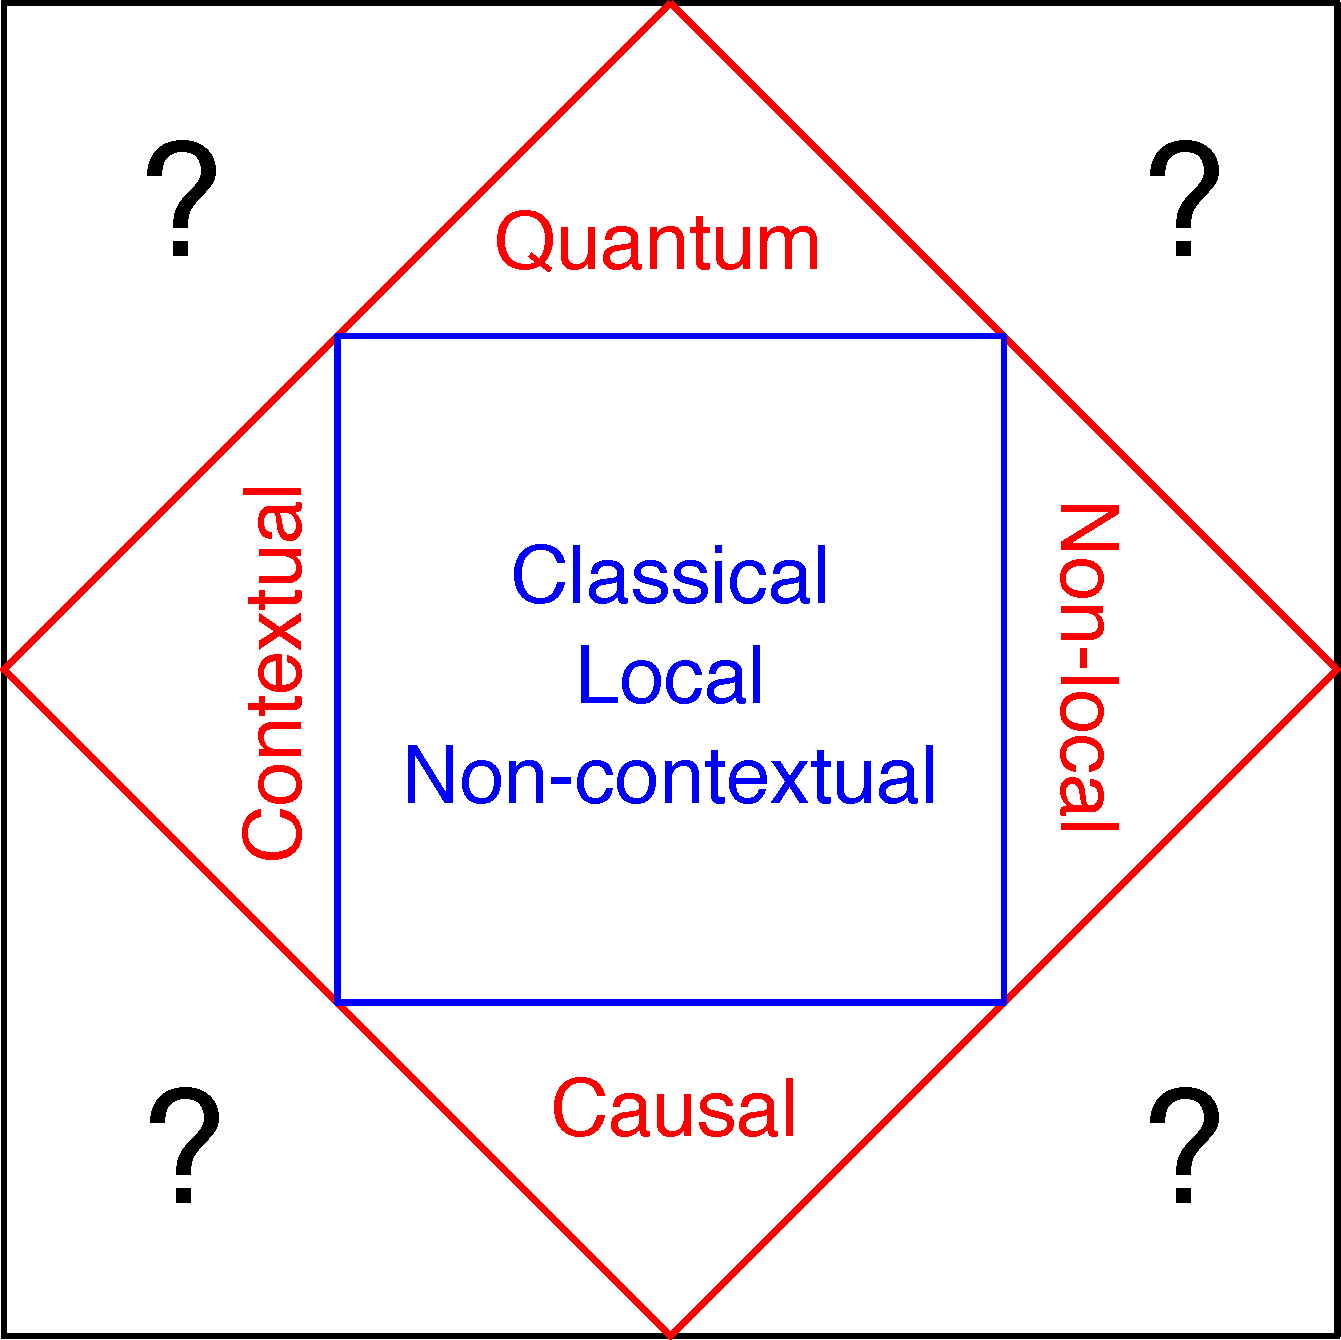
\includegraphics[width=2in]{quantum-yantra.pdf}
\caption{Schematic of the worlds of classical correlations, quantum correlations  and ``super-strong'' unphysical correlations}
\label{QYantra}
\end{center}
\end{figure}



\section{Measurements}
\label{sMeasure}
\subsection{What are the questions?}
\index{Measurement}
Up to now I have not  discussed much the question of quantum measurements.
I simply took the standard point of view that  (at least in principle) ideal projective measurements are feasible and one should look at the properties of the outcomes. 
The question is of course highly more complex. In this section I just recall some basic points about quantum measurements.


The meaning of the measurement operations is at the core of quantum physics. It was considered as such from the very beginning.
See for instance the proceedings of the famous Solvay 1927 Congress \cite{Solvay27}, and the 1983 review by Wheeler and Zurek \cite{WheelerZurek83}. Many great minds have thought about the so called ``measurement problem''  and the domain has been revived in the last decades by the experimental progresses, which allows now to manipulate simple quantum system and implement effectively ideal measurements.

On one hand, quantum measurements represent one of the most puzzling features of quantum physics. They are non-deterministic processes (quantum mechanics predicts only probabilities for outcomes of measurements). They are irreversible processes (the phenomenon of the ``wave-function collapse''). They reveal the irreducible uncertainty of quantum physics (the uncertainty relations).
This makes quantum measurements very different from ``ideal classical measurements''. 

On the other hand, quantum theory is the first physical theory that addresses seriously the problem of the interactions between the observed system (the object) and the measurement apparatus (the observer).
Indeed in classical physics the observer is considered as a spectator, able to register the state of the real world (hence to have its own state modified by the observation), but without perturbing the observed system in any way. 
Quantum physics shows that this assumption is not tenable. 
Moreover, it seems to provide a logically satisfying answer\footnote{If not satisfying every minds, every  times...} to the basic question: what are the minimal constraints put on the results of physical measurements by the basic physical principles\footnote{Well...  as long as gravity is not taken into account!}.

It is often stated that the main problem about quantum measurement is the problem of the uniqueness of the outcome. 
For instance, why do we observe a spin 1/2 (i.e. a q-bit) in the state $|{\uparrow}\rangle$ or in the state $|{\downarrow}\rangle$ when we start in a superposition $|\psi\rangle=\alpha|{\uparrow}\rangle+\beta |{\downarrow}\rangle$? However by definition a measurement is a process which gives one single classical outcome (out of several possible).
Thus in my opinion the real questions, related to the question of the ``projection postulate'', are: (1) Why do repeated ideal measurements should give always the same answer? 
(2) Why is it not  possible to ``measure'' the full quantum state $|\psi\rangle$ of a q-bit by a \emph{single} measurement operation, but only its projection onto some reference frame axis?

Again, the discussion that follows is very sketchy and superficial. A good recent reference, both on the history of the ``quantum measurement problem'', a detailed study of explicit dynamical models for quantum measurements, and a complete bibliography, is the research and review 
article \cite{AlBaNi2012}. 
\subsection{The von Neumann paradigm}
The general framework to discuss quantum measurements in the context of quantum theory is provided by J. von Neumann
\index{von Neumann J.}  in his 1932 book \cite{vonNeumann32G,vonNeumann32}.
\index{Non-destructive measurement}
\index{Ideal measurement}
Let me present it on the simple example of the q-bit.

But before, let me insist already on the fact that this discussion will not provide a derivation of the principle of quantum mechanics (existence of projective measurements, probabilistic features and Born rule), but rather a self-consistency argument of compatibility between the axioms of QM about measurements and what QM predicts about measurement devices.

An ideal measurement involves the interaction between the quantum system $\mathcal{S}$ (here a q-bit) and a measurement apparatus $\mathcal{M}$ which is a \emph{macroscopic object}.
The idea is that $\mathcal{M}$ must be treated as a quantum object, like $\mathcal{S}$.
An ideal non destructive measurement on $\mathcal{S}$ that does not change the orthogonal states  $|{\uparrow}\rangle$ and  $|{\downarrow}\rangle$ of $\mathcal{S}$ (thus corresponding to a measurement of the spin along the $z$ axis, $S_z$), correspond to introducing for a finite (short) time an interaction between $\mathcal{S}$ and $\mathcal{M}$, and to start from a well chosen initial state $|I\rangle$ for $\mathcal{M}$. The interaction and the dynamics of $\mathcal{M}$ must be such that, if one starts from an initial separable state where $\mathcal{S}$ is in a superposition state
\begin{equation}
\label{UMeasEv}
|\psi\rangle=\alpha\, |{\uparrow}\rangle+\beta\, |{\downarrow}\rangle
\end{equation}
after the measurement (interaction) the whole system (object+apparatus) is in an entangled state
\begin{equation}
\label{ }
|\psi\rangle\otimes |I\rangle\qquad\to\qquad\alpha\,|{\uparrow}\rangle\otimes |F_+\rangle + \beta\, |{\downarrow}\rangle\otimes|F_-\rangle
\end{equation}
The crucial point is that the final states $|F_+\rangle$ and $|F_-\rangle$ for $\mathcal{M}$ must be \emph{orthogonal} 
\footnote{as already pointed out in \cite{vonNeumann32G}   }

\begin{equation}
\label{ }
\langle F_+ | F_-\rangle=0
\end{equation}
Of course this particular evolution \ref{UMeasEv} is unitary for any choice of $|\psi\rangle$, since it transforms a pure state into a pure state.
\begin{equation}
\label{vNDecProj}
|\psi\rangle\otimes |I\rangle
\qquad\to\qquad
\alpha\,|{\uparrow}\rangle\otimes |F_+\rangle + \beta\, |{\downarrow}\rangle\otimes|F_-\rangle
\end{equation}

One can argue that this is sufficient to show that the process has all the characteristic expected from an ideal measurement, within the quantum formalism itself. Indeed, using the Born rule, this is consistent with the fact that the state $\alpha|{\uparrow}\rangle$ is observed with probability $p_+=|\alpha|^2$ and the state $\alpha|{\downarrow}\rangle$ with probability $p_-=|\beta|^2$. 
Indeed the reduced density matriices both for the system $\mathcal{S}$ and for the system $\mathcal{M}$ (projected onto the two pointer states) is that of a completely mixed state
\begin{equation}
\label{ }
\rho_\mathcal{S}=
\begin{pmatrix}
   p_+   &    0\\
   0   &  p_-
\end{pmatrix}
\end{equation}

For instance, as discussed in   \cite{vonNeumann32G}\cite{vonNeumann32}, if one is in the situation where the observer $\mathcal{O}$, really observe the measurement apparatus $\mathcal{M}$, not the system $\mathcal{S}$ directly, the argument can be repeated as
\begin{equation}
\label{ }
|\psi\rangle\otimes |I\rangle\otimes |O\rangle
\qquad\to\qquad
\alpha\, | {\uparrow}\rangle \otimes |F_+\rangle \otimes |O_+\rangle + \beta\,  |{\downarrow}\rangle\otimes|F_-\rangle \otimes |O_-\rangle
\end{equation}
and it does not matter if one puts the fiducial separation between object and observer between $\mathcal{S}$ and $\mathcal{M}+\mathcal{O}$ or between $\mathcal{S}+\mathcal{M}$ and $\mathcal{O}$. This argument being repeated ad infinitum.

A related argument is that once a measurement has been performed, if we repeat it using for instance another copy $\mathcal{M}'$ of the measurement apparatus, after the second measurement we obtain
\begin{equation}
\label{ }
|\psi\rangle\otimes |I\rangle\otimes |  I' \rangle\qquad\to\qquad\alpha\, |{\uparrow}\rangle\otimes |F_+\rangle \otimes |F'_+\rangle+ \beta \, |{\downarrow}\rangle\otimes|F_-\rangle\otimes|F'_-\rangle
\end{equation}
so that we never observe both  $|{\uparrow}\rangle$ and  $|{\downarrow}\rangle$ in a successive series of measurements (hence the measurement is really a projective measurements). 
The arguments holds also if the outcome of the first measurement is stored on some classical memory device $\mathcal{D}$ and the measurement apparatus reinitialized to $|I\rangle$.
This kind of argument can be found already in 
\cite{Mott29}.

The discussion here is clearly outrageously oversimplified and very sketchy. For a  precise discussion, one must distinguish among the degrees of freedom of the measurement apparatus $\mathcal{M}$ the (often still macroscopic) variables which really register the state of the observed system, the so called\emph{ pointer states}, from the other (numerous) microscopic degrees of freedom of $\mathcal{M}$, which are present anyway since $\mathcal{M}$ is a macroscopic object, and which are required both for ensuring decoherence (see next section) and to induce dissipation, so that the pointer states become stable and store in a efficient way the information about the result of the measurement. One must also take into account the coupling of the system $\mathcal{S}$ and of the measurement apparatus $\mathcal{M}$ to the environment $\mathcal{E}$.

\subsection{Decoherence and ergodicity (mixing)}
As already emphasized, the crucial point is that starting from the same initial state $|I\rangle$, the possible final pointer states for the measurement apparatus, $|F_+\rangle$ and $|F_-\rangle$, are orthogonal. 
This is now a well defined dynamical problem, which can be studied using the theory of quantum dynamics for closed and open systems. The fact that $\mathcal{M}$ is macroscopic, i.e. that its Hilbert space of states in very big, is essential, and the crucial concept is  \emph{decoherence} (in a general sense).

\index{Decoherence}
The precise concept and denomination of quantum decoherence was introduced in the 70's (especially by Zeh) and developed and popularized in the 80's (see the reviews
\cite{JoosZehKiefer2003}, \cite{Zurek2003}). But the basic idea seems much older and for our purpose one can probably go back to the end of the 20' and to von Neumann's 
\index{von Neumann J.}
 quantum ergodic theorem \cite{vonNeumann29} (see \cite{springerlink:10.1140/epjh/e2010-00008-5} for the english translation and \cite{GoldLebMasTumZan2010} for historical and physical perspective).
\index{Quantum ergodic theorem}

One starts from the simple geometrical remark \cite{vonNeumann29} that if $| e_1 \rangle$ and $| e_2 \rangle$ are two \emph{random 
unit vectors }in a $N$ dimensional Hilbert space $\mathcal{H}$ (real or complex), their average ``overlap'' (squared scalar product) is of order
\begin{equation}
\label{ }
\overline{|\langle e_1 | e_2 \rangle  |^2}\ \simeq {1\over N}
\quad,\qquad N=\dim (\mathcal{H})
\end{equation}
hence it is very small, and for all practical purpose equal to $0$, if $N$ is very large. Remember that for a quantum system made out of $M$ similar subsystems, $N\propto (N_0)^M$, $N_0$ being the number of accessible quantum states for each subsystem.

A simple idealized model to obtain a dynamics of the form \ref{vNDecProj} for $\mathcal{S}+\mathcal{M}$ is to assume that both $\mathcal{S}$ and $\mathcal{M}$ have no intrinsic dynamics and that the evolution during the interaction/measurement time interval is given by a interaction Hamiltonian (acting on the Hilbert space $\mathcal{H}=\mathcal{H}_\mathcal{S}\otimes\mathcal{H}_\mathcal{M}$ of $\mathcal{S}+\mathcal{M}$)  of  the form
 \begin{equation}
\label{Hdec}
H_\mathrm{int}=  |  {\uparrow}\rangle \langle {\uparrow} |  \otimes  H_+ +  |  {\downarrow}\rangle \langle  {\downarrow} |  \otimes  H_-
\end{equation}
where $H_+$ and $H_-$ are two \emph{different} Hamiltonians (operators) acting on $\mathcal{H}_\mathcal{M}$.
It is clear that if the interaction between $\mathcal{S}$ and $\mathcal{M}$ takes place during a finite time $t$, and is then switched off, the final state of the system is an entangled one of the form \ref{vNDecProj}, with
\begin{equation}
\label{F+F-Exp}
|F_+ \rangle = \emath^{{t\over \imath\hbar} H_+} |I\rangle
\quad,\qquad
|F_- \rangle = \emath^{{t\over \imath\hbar} H_-} | I \rangle
\end{equation}
so that
\begin{equation}
\label{F+F-Overlap}
\langle F_+|F_-\rangle = \langle I | \emath^{-{t\over \imath\hbar} H_+} \cdot\emath^{{t\over \imath\hbar} H_-} |I\rangle
\end{equation}
It is quite easy to see that if $H_+$ and $H_-$ are not (too much) correlated (in a sense that I do not make more precise), the final states $|F_+\rangle$ and $|F_-\rangle$ are quite uncorrelated with respect to each others and with the initial state $|I\rangle$  after a very short time, and may be considered as random states in $\mathcal{H}_\mathcal{M}$, so that 
\begin{equation}
\label{F+F-OSm}
|\langle F_+|F_-\rangle|^2\simeq {1\over\dim(\mathcal{H}_\mathcal{M})}\ll\!\! \ll 1
\end{equation}
so that for all practical purpose, we may assume that
\begin{equation}
\label{F+F-zero}
\langle F_+ | F_-\rangle =0
\end{equation}
This is the basis of the general phenomenon of \emph{decoherence}. 
The interaction between the observed system and the measurement apparatus has induced a decoherence between the states $|\uparrow\rangle$ and $| \downarrow \rangle$ of $\mathcal{S}$, but also a decoherence between the pointer states $| F_+\rangle$ and $| F_-\rangle$ of $\mathcal{M}$.

Moreover, the larger $\dim(\mathcal{H}_\mathcal{M})$, the smaller the ``decoherence time'' beyond which $\langle F_+ | F_-\rangle \simeq 0$ is (and it is often in practice too small to be observable), and the larger (in practice infinitely larger)  the ``quantum Poincar\'{e} recurrence  time'' (where one might expect to get again $|\langle F_+ | F_-\rangle| \simeq  1$) is.


Of course, as already mentionned, this is just the first step in the discussion of the dynamics of a quantum measurement. One has in particular to check and to explain how, and under which conditions, the pointer states are quantum microstates which correspond to macroscopic classical-like macrostates, which can be manipulated, observed, stored in an efficient way. 
At that stage, I just paraphrase J. von Neumann (in the famous  chapter VI  ``Der Me\ss proze\ss '' of  \cite{vonNeumann32G})
\begin{center}
\emph{``Die weitere Frage (...) soll uns dagegen nicht besch\"{a}ftigen.''}
\end{center}

Decoherence is a typical quantum phenomenon. It explains how, in most situations and systems, quantum correlations in small (or big) multipartite systems are ``washed out" and disappear through the interaction of the system with other systems, with its environment or its microscopic  internal degrees of freedom. 
Standard references on decoherence and the general problem of the quantum to classical transitions are  \cite{Zurek:1990fk} and\cite{Schlosshauer07}.

However, the underlying mechanism for decoherence has a well know classical analog: it is the (quite generic) phenomenon of \emph{ergodicity}, or more precisely the \emph{mixing property} of classical dynamical systems.
\index{Ergodicity}
I refer to textbooks such as \cite{ArnoldAvez-book68} and \cite{LichLieb-book92} for precise mathematical definitions, proofs and details. 
Again I give here an oversimplified presentation.

Let us consider a classical Hamiltonian system. One considers its dynamics on (a fixed energy slice $H=E$ of) the phase space $\Omega$ , assumed to have a finite volume $V=\mu(\Omega)$ normalized to $V=1$,  where $\mu$ is the Liouville measure. 
We denote $T$ the volume preserving  map $\Omega\to\Omega$ corresponding to the integration of the Hamiltonian flow during some reference time $t_0$. $T^k$ is the iterated map (evolution during time $t=k t_0$). This discrete time dynamical mapping given by $T$ is said to have the \emph{weak mixing property} if for any two (measurable) subsets $A$ and $B$ of $\Omega$ one has
\index{Mixing property}
\begin{equation}
\label{ }
\lim_{n\to\infty} \  {1\over n}\sum_{k=0}^{n-1} \mu(B\cap T^k A)  \ =\ \mu(B)\mu(A)
\end{equation}
The (weak) mixing properties means (roughly speaking)  that, if we take a random point $a$  in phase space, its iterations $a_k=T^k a$ are at large time and ``on the average'' uniformly distributed on phase space, with a probability $\mu(B)/\mu(\Omega)$ to be contained inside any subset $B\in\Omega$.
See fig.~\ref{fWMixing}
\begin{figure}[h]
\begin{center}
%\vskip -4ex \hskip 4 em
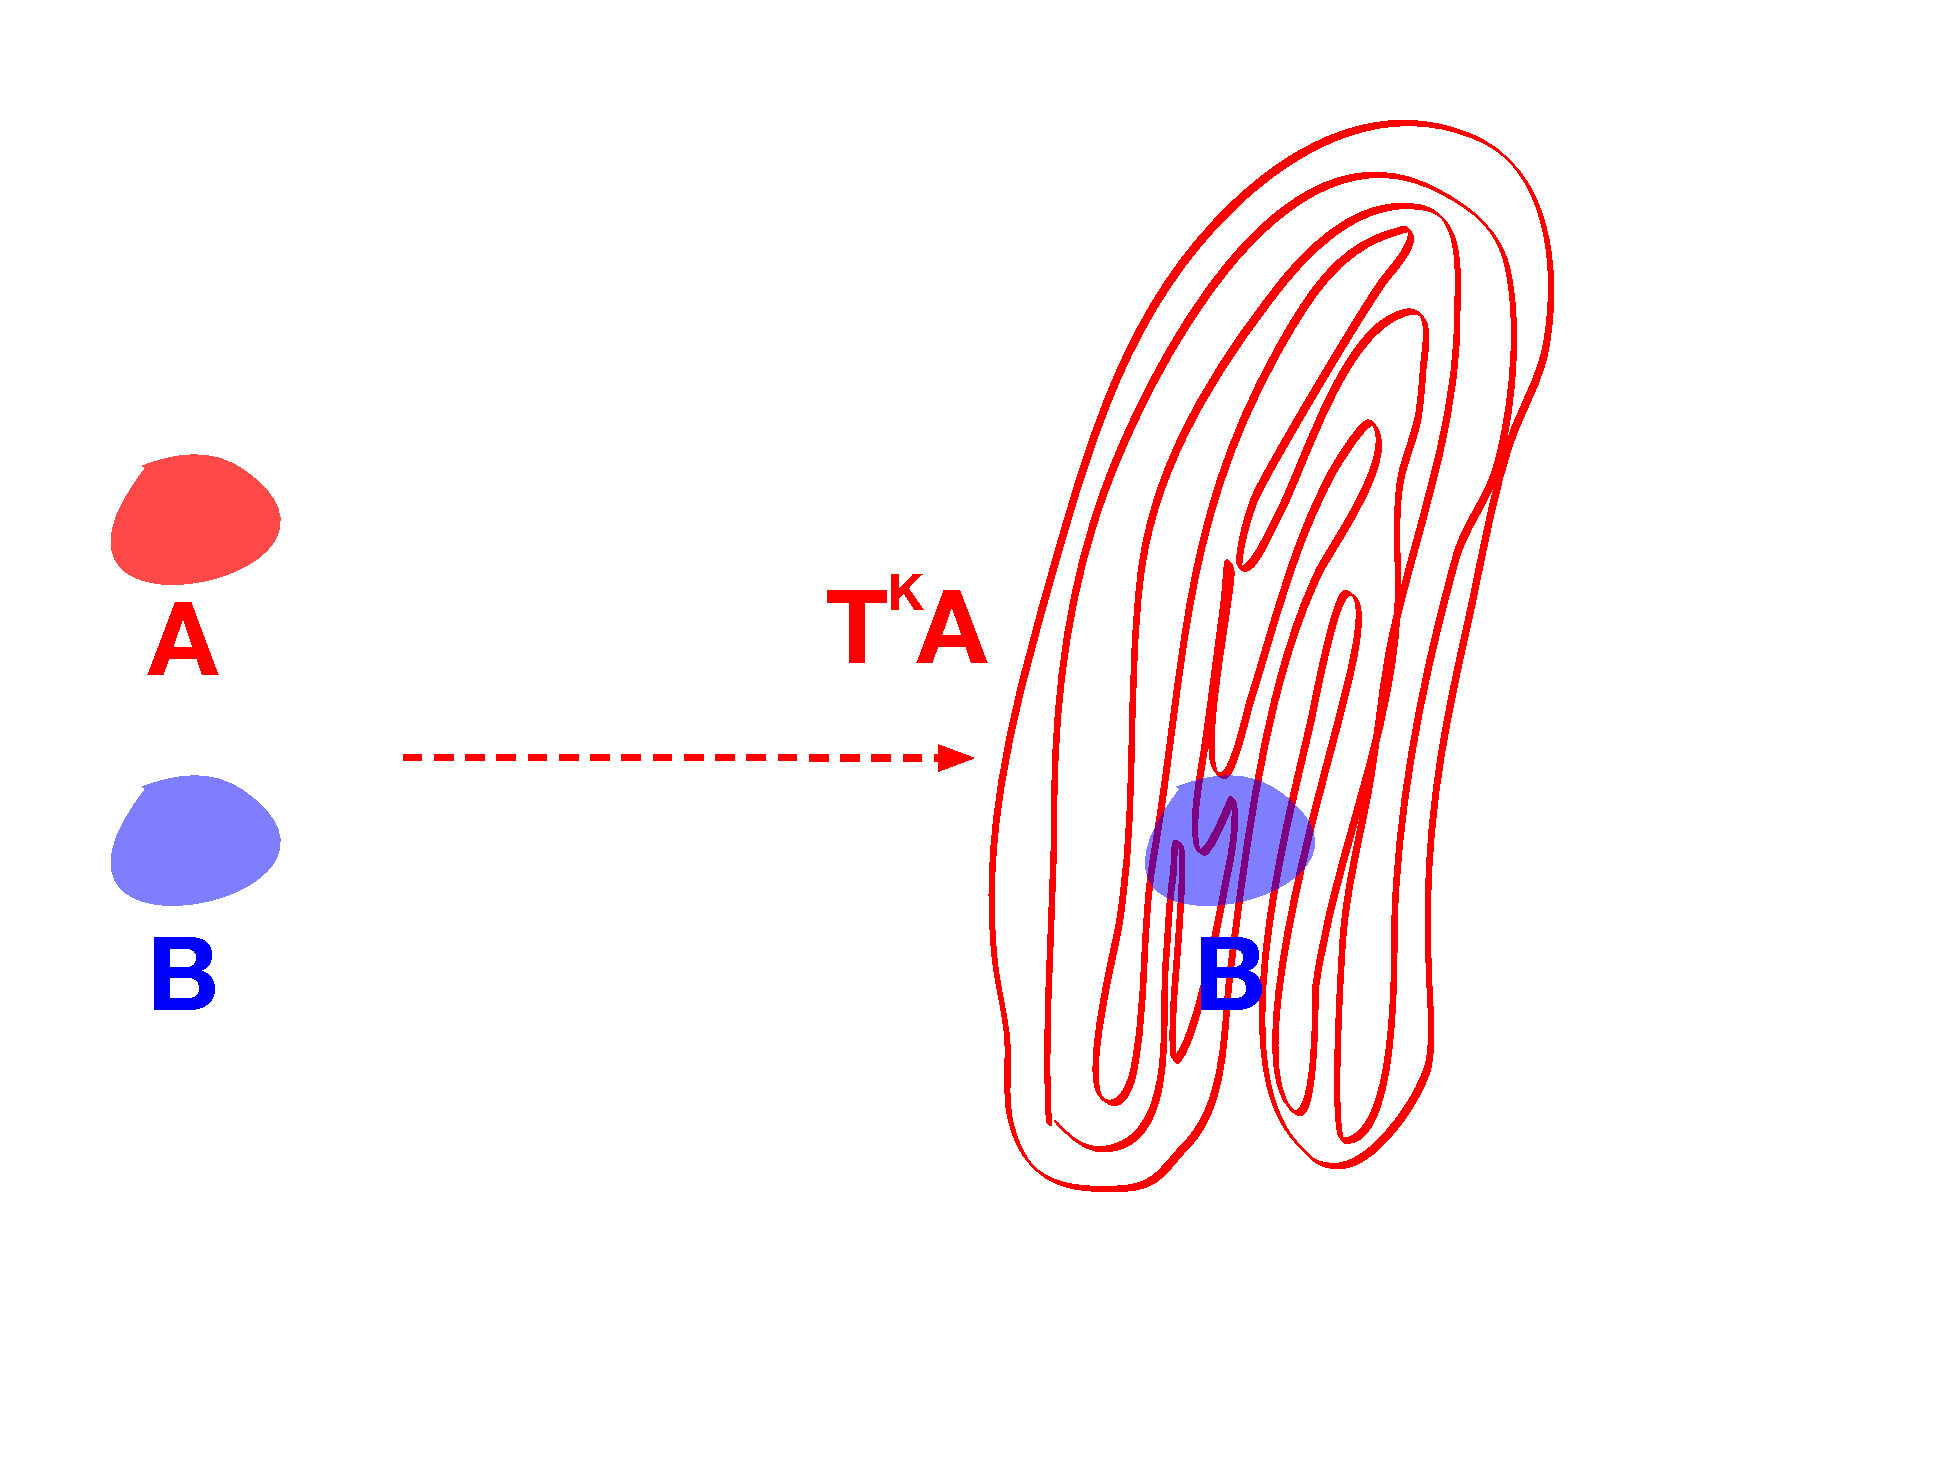
\includegraphics[height=2.in]{Mixing.pdf}
%\vskip -4ex 
\caption{Graphical representation of the mixing property (very crude)}
\label{fWMixing}
\end{center}
\end{figure}

Weak mixing is one of the weakest form of ``ergodicity'' (in a loose sense, there is a precise mathematical concept of ergodicity).

Now in semiclassical quantization (for instance using Bohr-Sommerfeld quantization rules)  if a classical system has $M$ independent degrees of freedom (hence its classical phase space $\Omega$ has dimension $2M$), the ``quantum element of phase space'' $\delta\Omega$ has volume $\delta V=\mu(\delta\Omega)= h^{M}$ with $h=2\pi\hbar$ the Planck's constant.
If the phase space is compact with volume $\mu(\Omega)<\infty$ the number of ``independent quantum states'' accessible to the system is of order $N=\mu(\Omega)/\mu(\delta\Omega)$ and should correspond to the dimension of the Hilbert space $N=\dim(\mathcal{H})$.
In this crude semiclassical picture, if we consider two pure quantum states $|a\rangle$ and $|b\rangle$ and associate to them two minimal semiclassical subsets $A$ and $B$ of the semiclassical phase space $\Omega$, of quantum volume $\delta V$, the semiclassical volume $\mu(A\cap B)$ corresponds to the overlap between the two quantum pure states through
\begin{equation}
\label{ }
\mu(A\cap B)\  \simeq \ {1 \over N} | \langle a |b\rangle |^2
\end{equation}
More generally if we associate to any (non minimal) subset $A$ of $\Omega$ a mixed state given by a quantum density matrix $\rho_A$ we have the semiclassical correspondence
\begin{equation}
\label{ }
{\mu(A\cap B)\over \mu(A)\mu(B)}\  \simeq\  {N}\   \tr(\rho_A\, \rho_B)
\end{equation}
With this semiclassical picture in mind (Warning! It does not work for all states, only for states which have a semiclassical interpretation! But pointer states usually do.) the measurement/interaction process discussed above has a simple semiclassical interpretation, illustrated on fig.~\ref{fFFMixing}. 

\begin{figure}[h]
\begin{center}
%\vskip -4ex
%\hskip 3 em
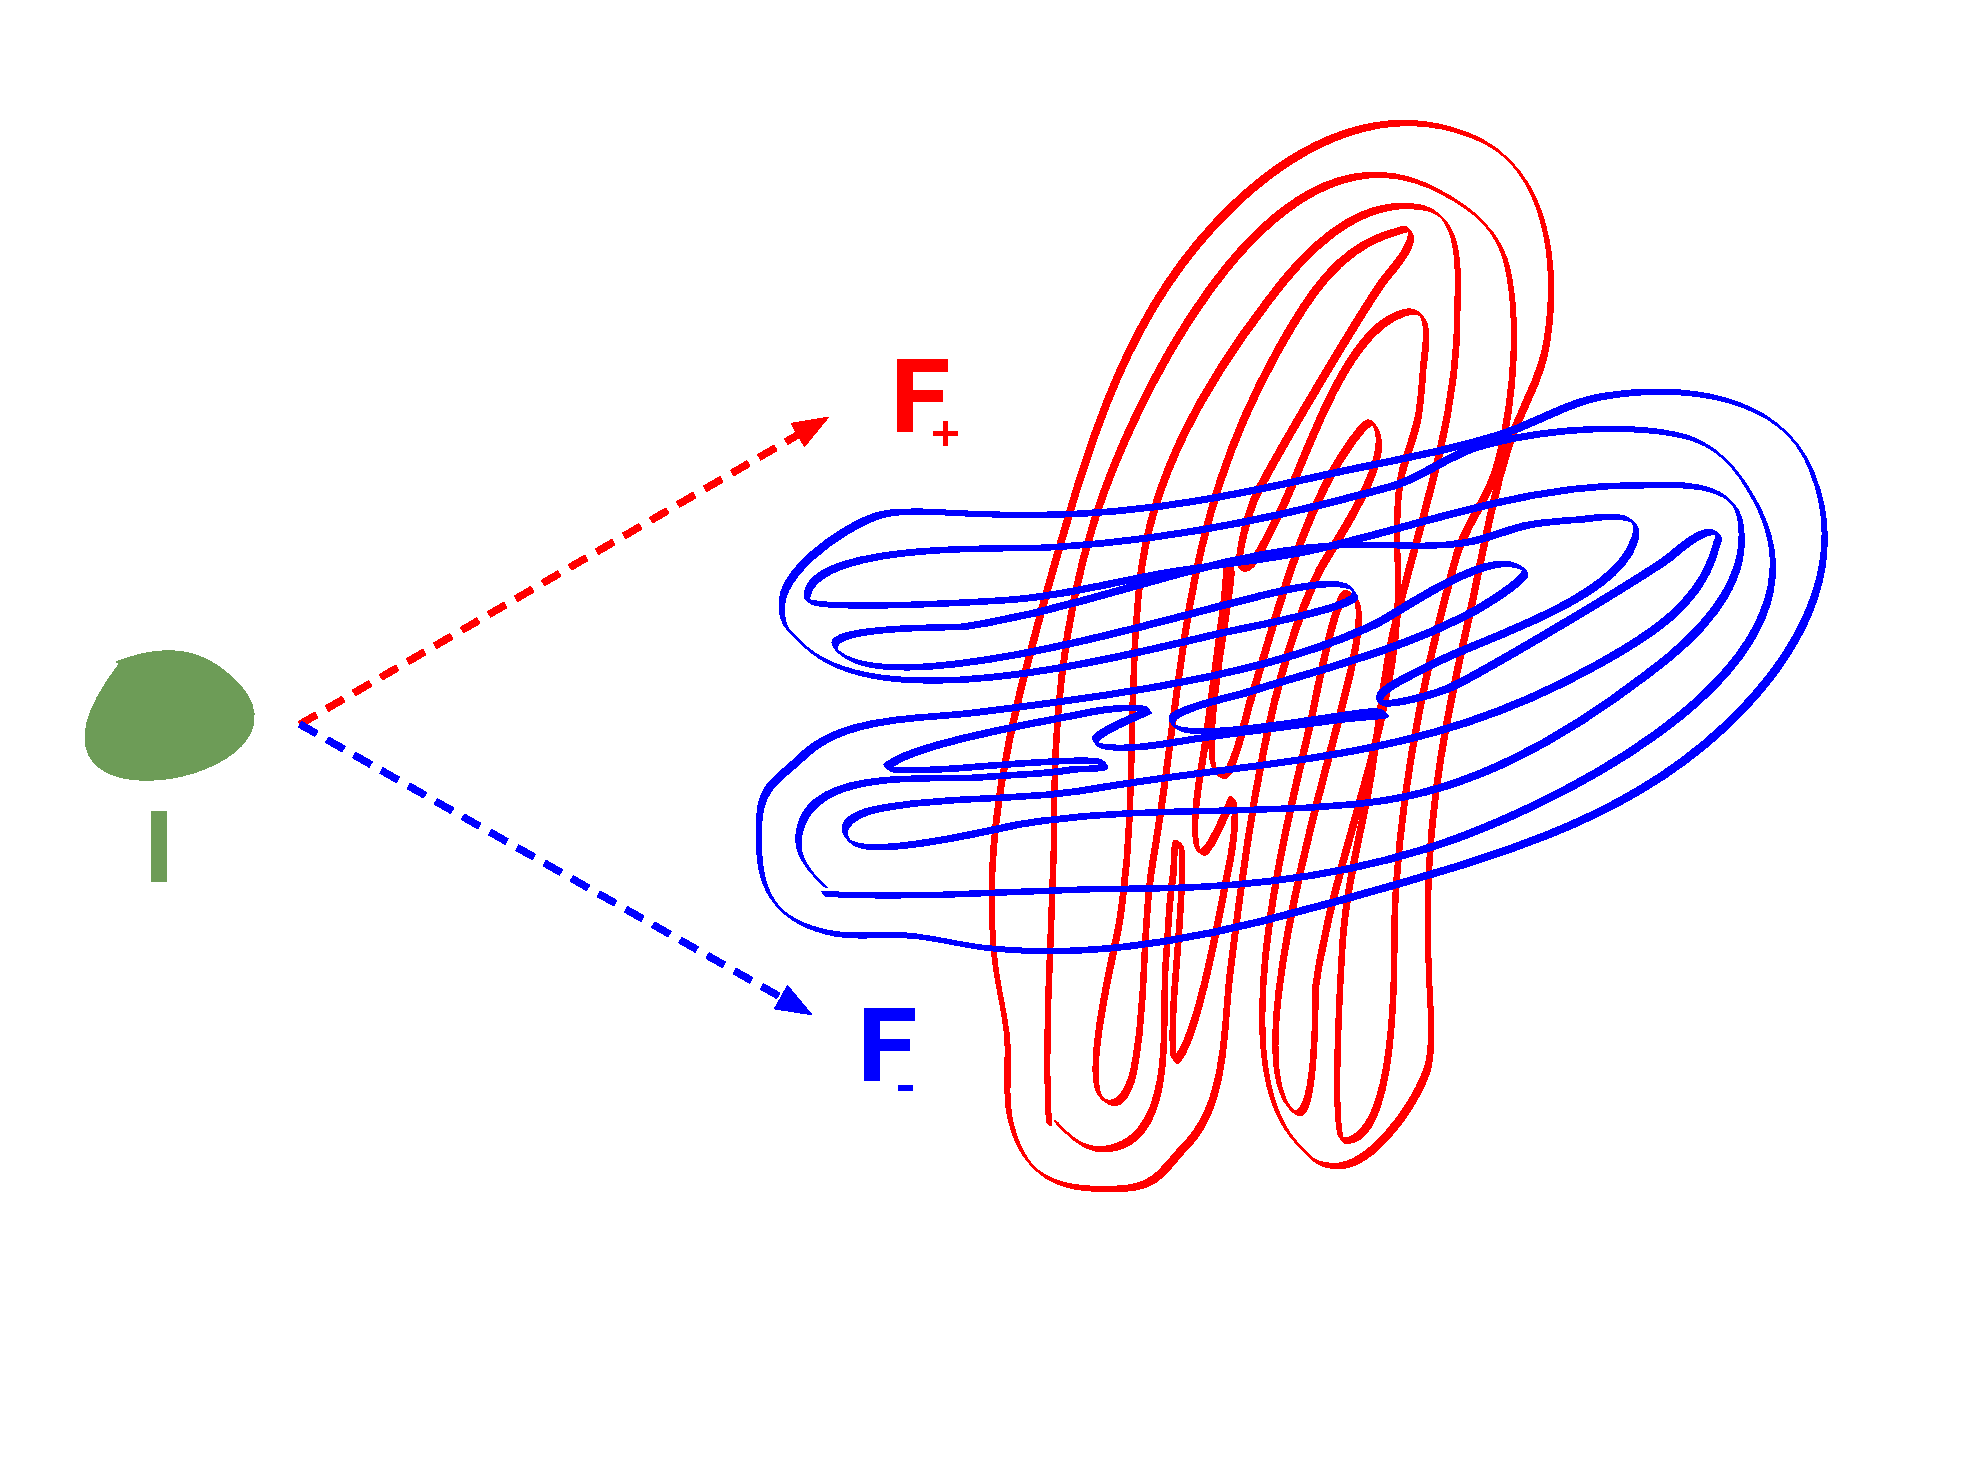
\includegraphics[height=2in]{Mixing-2.pdf}\qquad\qquad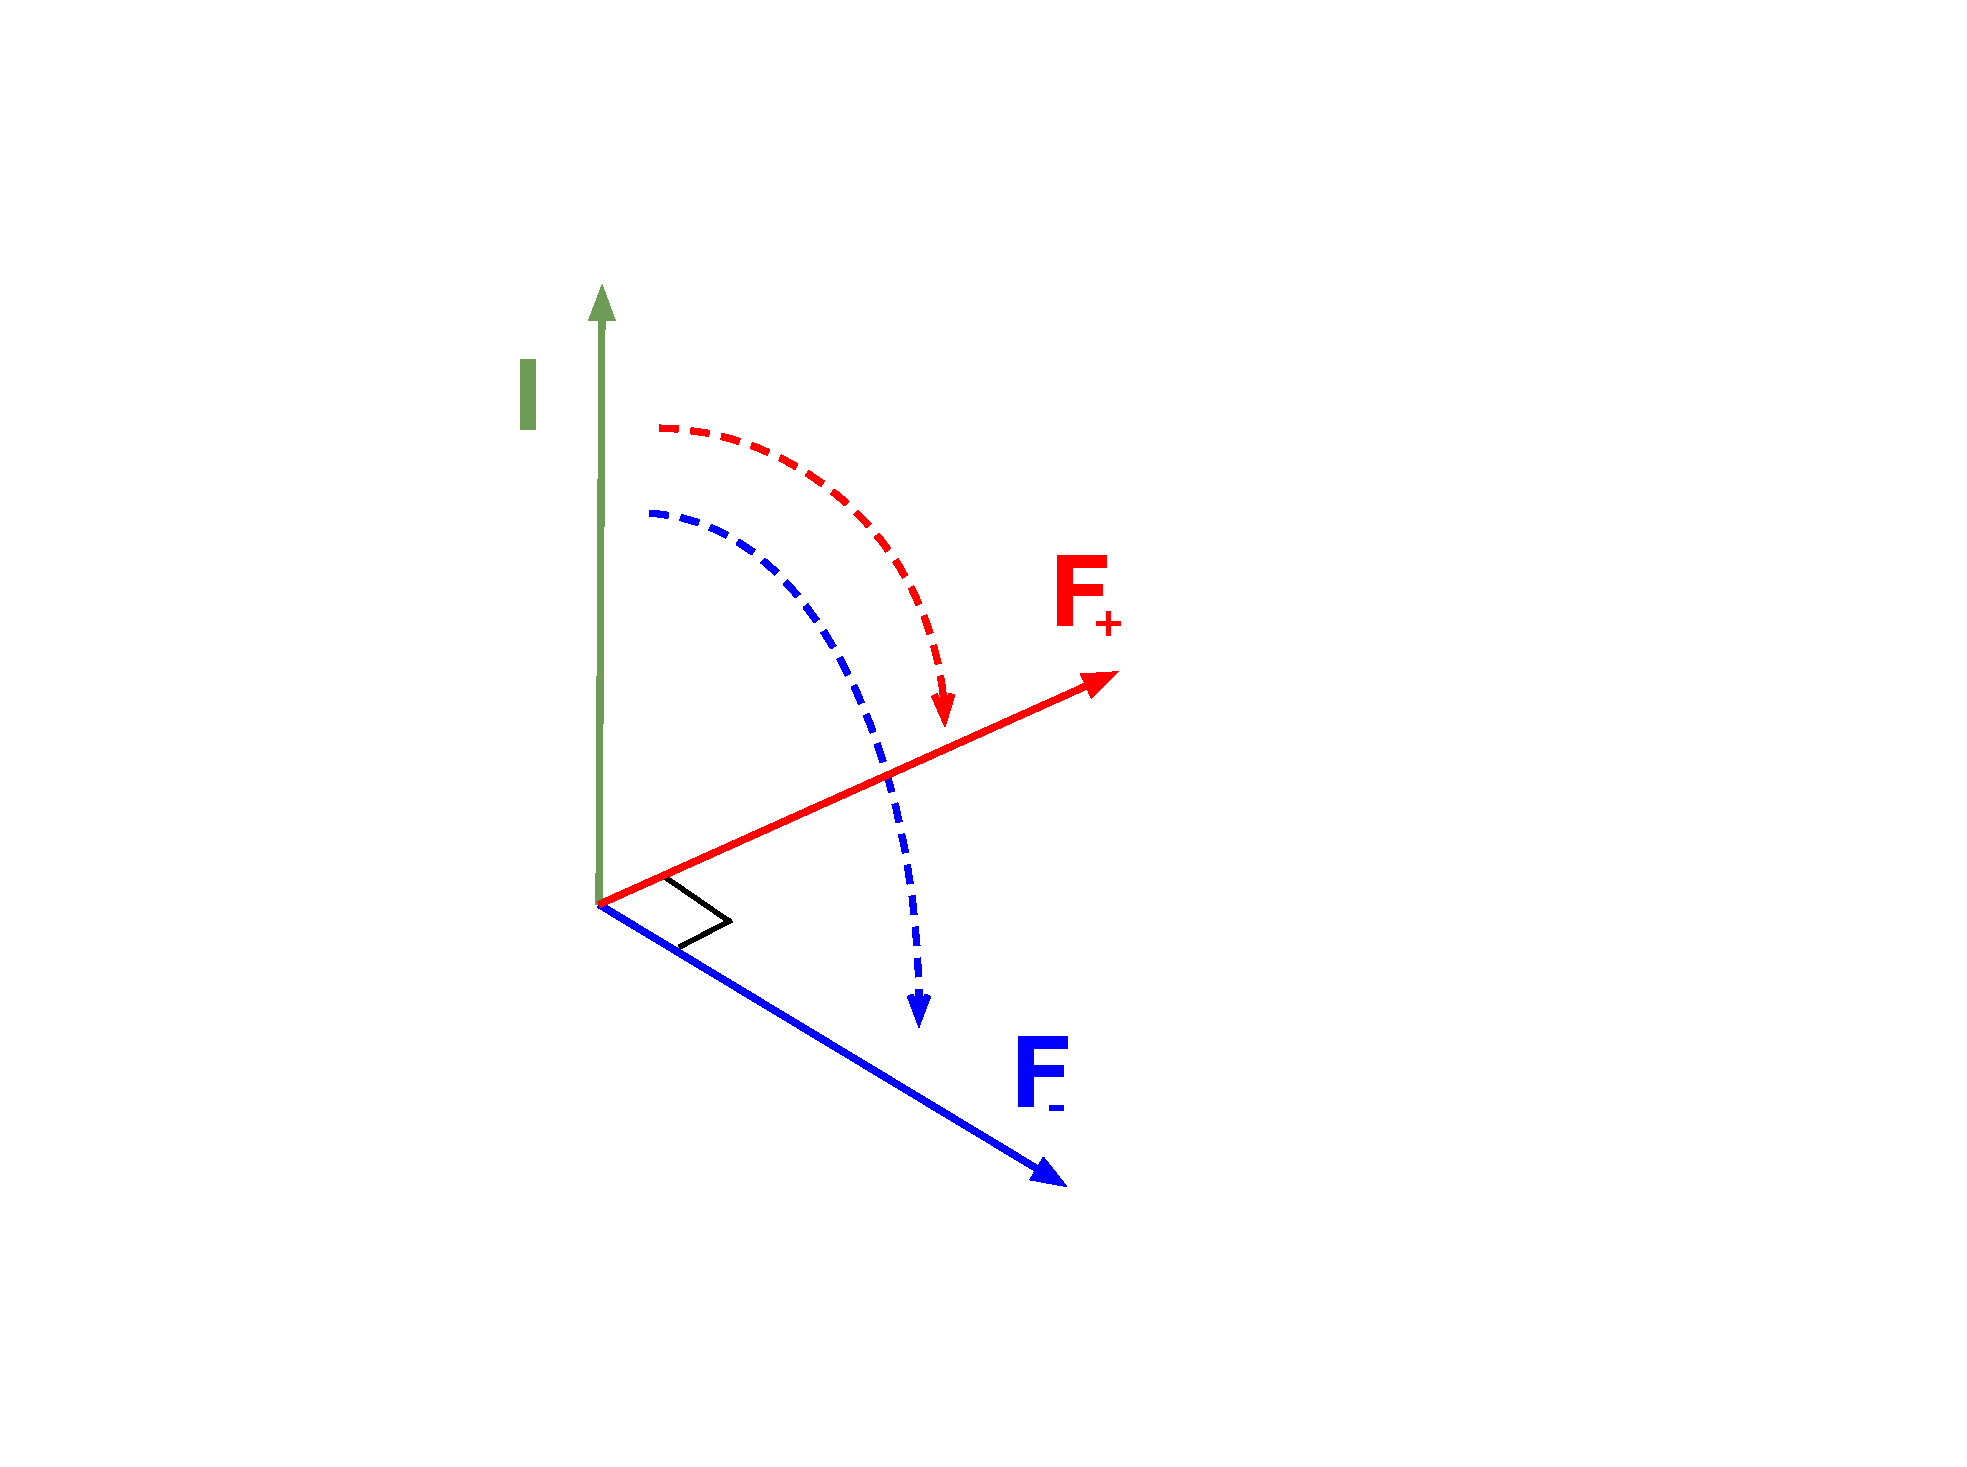
\includegraphics[height=2in]{MixingQ.pdf}
%\vskip -4ex
\caption{Crude semiclassical and quantum pictures of the decoherence process \ref{F+F-Exp}-\ref{F+F-OSm}}
\label{fFFMixing}
\end{center}
\end{figure}

The big system $\mathcal{M}$ starts from an initial state $|I\rangle$  described by a semiclassical element $I$. 
If the system $\mathcal{S}$ is in the state $|\uparrow\rangle$, $\mathcal{M}$ evolves to a state $| F_+\rangle$ corresponding to $F_+$.
If it is in the state $|\uparrow\rangle$, $\mathcal{M}$ evolves to a state $| F_-\rangle$ corresponding to $F_-$.
For well chosen, but quite generic Hamiltonians $H_+$ and $H_-$, the dynamics is mixing, so that, while $\mu(F_+)=\mu(F_-)=1/N$, typically one has $\mu(F_+\cap F_-)=\mu(F_+) \mu(F_-) = 1/N^2\ll 1/N$.
Thus it is enough for the quantum dynamics generated by $H_+$ and $H_-$ to have a quantum analog the classical property of mixing, which is quite generic, to ``explain'' why the two final states $|F_+\rangle$ and $|F_-\rangle$ are generically (almost) orthogonal.

\subsection{Discussion}
As already stated, the points that I tried to discuss in this section represent only a small subset of the questions about measurements in quantum mechanics. Again, I refer for instance to \cite{AlBaNi2012} and \cite{Laloe-book} (among many other reviews) for a serious discussion and bibliography.

I have not discussed more realistic measurement processes, in particular the so called ``indirect measurements procedures'', or ``weak measurements'', where the observations on the system are performed through successive interactions with other quantum systems (the probes) which are so devised as to perturb as less as possible the observed system, followed by stronger direct (in general destructive) measurements of the state of the probes.
Such measurement processes, as well as many interesting questions and experiments in quantum physics, quantum information sciences, etc. are described by the general formalism of POVM's (Positive Operator Valued Measure). I do not discuss these questions here.
\index{Indirect measurements}
\index{POVM}

In any case,  important aspects of quantum measurements belong to the general class of problems of the emergence and the meaning of irreversibility out of reversible microscopic laws in physics (quantum as well as classical). See for instance 
\cite{Halliwell96}.

The quantum formalism as it is presented in these lectures starts (amongst other things) from explicit assumptions on the properties of measurements. The best one can hope is to show that the quantum formalism is consistent: the characteristics and behavior of (highly idealized) physical measurement devices, constructed and operated according to the laws of quantum mechanics, should be consistent with the initials axioms. 

One must be careful however, when trying to justify or rederive some of the axioms of quantum mechanics from the behavior of measurement apparatus and their interactions with the observed system and the rest of the world, not to make circular reasoning. 


\section{Interpretations versus Alternative Theories }

In these notes I have been careful not to discuss the interpretation issues of quantum mechanics.
There are at least two reasons.
\begin{enumerate}
  \item These notes are focused on the mathematical formalism of ``standard quantum mechanics". Thus I adopt the ``operational'' point of view
\footnote{This is probably the point of view adopted by most physicists, chemists, mathematicians, computer scientists, engineers, ...  who deal with the quantum world.}
that quantum mechanics is a theoretical framework which provides rules to compute the probabilities to obtain a given result when measuring some observable of a system in a given state.  The concepts of ``observables'', ``states'' and ``probabilities'' being defined through the principles (axioms in a non-mathematical sense) of the formalisms considered.
  \item I do not feel qualified enough to discuss  all the interpretations that have been proposed  and all the philosophical questions raised by quantum physics since its birth. This does not mean that these question are unimportant.
 \end{enumerate}
 However, let me just make a few simple, and probably naive,  remarks.
 
 
Many interpretations of quantum mechanics do not challenge the present standard mathematical formulations of the theory.
They rather insist on a particular point of view or a particular formulation of quantum mechanics as the best suited or the preferable one to consider and study quantum systems, and the quantum world.
They may be considered as particular choices
 \footnote{This does not mean that I am an adept of some post-modern relativism...}
 of  point of view and of  philosophical option to think about quantum mechanics and practice it.
 
 
 This is clearly the case for the so-called Copenhagen interpretations. 
 \index{Copenhagen interpretation}
 They insist on the fact that QM deals only with predictions for results of operations, and they can be considered as ``quantum mechanics from a strong pragmatist 
 \footnote{In the philosophical sense of pragmatism}
 point of view".
Remember however that there is no clear cut definition of what a Copenhagen interpretation is. The term was introduced only in 1955 by Heisenberg. I refer to the paper by Howard \cite{Howard2004} for an historical and critical review of the history, uses and misuses of the concept.
\index{Many world interpretation}
 This is also  the case for the ``many worlds interpretations'', that tries to take seriously the concept of ``wave function of the universe''. 
They can be considered (when used reasonably for physics) as the other extreme of ``quantum mechanics from a strong realist 
 \footnote{In the philosophical sense of realism}
 point of view".
 Again there are many variants of these kind of interpretations. I refer to \cite{MWDeWittGraham73} for  the original papers, and to \cite{MW2010} for a recent  presentation of the subject and contradictory discussions.
 
 There is a whole spectrum of  proposed interpretations, for instance the ``coherent history formulations" and the ``modal interpretations'' . I do not  discuss these interpretations here.
 
 The interpretations that rely on the mathematical formulations of quantum mechanics should be clearly distinguished
 \footnote{This is unfortunately not always the case in popular -- and even in some advanced -- presentations and discussions of quantum physics.}
  from another class of  proposals to explain quantum physics that rely on modifications of the rules and are different physical theories. 
These modified or alternative quantum theories  deviate from ``standard'' quantum mechanics and should be experimentally falsifiable (and sometimes are already falsified).

\index{Hidden variables}
This is the case of the various non-local hidden-variables proposals, such as the de Broglie-Bohm theory, which contain some variables (degrees of freedom) which do not obey the laws of QM, and which cannot be observed directly. One might think that they are not falsifiable, but remember that there are serious problems from contextuality, which means that in general, if one want to keep non-contextuality, not all physical (i.e. that can be measured) observables are expected to behave as QM predicts.


\index{Collapse models}
This is also the case for the class of models known as ``collapse models''. 
See \cite{GhRiWe1985,GhRiWe1986} for the first models.
In these models the quantum dynamics is modified (for instance by non-linear terms) so that the evolution of the wave functions is not unitary any more (while the probabilities are conserved of course), and the ``collapse of the wave function'' is a dynamical phenomenon. 
 These models are somehow phenomenological and of course not (yet?) fully  internally consistent, since the origin of these non linear dynamics is quite ad hoc. 
 They predict a breakdown of the law of QM for the evolution of quantum coherences and decoherence phenomenon at large times, large distances, or in particular for big quantum systems (for instance large molecules or atomic clusters).  
At the present day, despite the impressive experimental progresses in the control of quantum coherences, quantum measurements, study of decoherence phenomenon, manipulation of information in quantum systems, etc. , no such violations of the predictions of standard QM and of unitary dynamics have been observed.
 
\section{What about gravity?}
Another really big subject that I do not discuss in these lecture is quantum gravity. Again just a few trivial remarks.
\index{Quantum gravity}

It is clear that the principles of quantum mechanics are challenged by the question of quantizing gravity. 
The challenges are not only technical. General relativity (GR) is indeed a non-renormalizable theory, and from that point of view a first and natural idea is to consider it as an effective low energy theory. After all, in the development of nuclear and particle physics (in the 30', the 40', the 60'...)  there have been several theoretical false alerts and clashes between experimental discoveries and the theoretical understanding that led many great minds to question the principles of quantum mechanics. However QM came out unscathed and even stronger, and since the 70' its principles are not challenged any more.

However with gravity the situation is different.  For instance the discovery of the Bekenstein-Hawking entropy of black holes, of the Hawking radiation, and of the ``information paradox'' shows that  fundamental questions remain to be understood about the relation between  quantum mechanics and the GR concepts of space and time. Indeed even the most advanced quantum theories available, quantum field theories such as non-abelian gauge theories
the standard model, its supersymmetric and/or grand unified extensions, still rely on the special relativity concept of space-time, or to some extend to the dynamical but still classical concept of curved space-time of GR.
It is clear that a quantum theory of space time will deeply modify, and even abolish, the classical concept of space-time as we are used to.
One should note two things. 

Firstly, the presently most advanced attempts to build a quantum theory incorporating gravity, namely string theory and its modern extensions, as well as the alternative approaches to build a quantum theory of space-time such as loop quantum gravity (LQG) and spin-foam models (SF), rely mostly on the quantum formalism as we know it, but change the fundamental degrees of freedom (drastically and quite widely for string theories, in a more conservative way for LQG/SF).
The fact that  string theories offers some serious hints of solutions of the information paradox, and some explicit solutions and ideas, like holography and AdS/CFT dualities, for viewing space-time as emergent, is a very encouraging fact.

Secondly, in the two formalisms presented here, the algebraic formalism and the quantum logic formulations, it should be noted that space and time (as  continuous entities)  play a secondary role with respect to the concept of causality and locality/separability. I hope this is clear in the way I choose to present the algebraic formalism in section \ref{s:AlgQM} and quantum logic in section \ref{s:QuanLog}. 
Of course space and time are essential for constructing physical theories out of the formalism.
Nevetheless, the fact that it is causal relations and causal independence between physical measurement operations that are essential for the formulation of the theory is also a very encouraging fact.

Nevertheless, if for instance the information paradox is not solved by a quantum theory of gravity, or if the concepts of causality and separability have to be rejected (for instance if no repeatable measurements are possible, and if no two sub-systems/sub-ensembles-of-degrees-of-freedom can be considered as really separated/independent), then one might expect that the basic principles of quantum mechanics will not survive (and, according to the common lore, should  be replaced by something even more bizarre and inexplicable...).

Well! It is time to end this bar room discussion.



